\subsection*{}
\section{Calibration en énergie des jets}

\begin{frame}
\begin{minipage}[t]{.45\textwidth}
\begin{center}
\manip Niveaux de connaissance

\vspace{.5\baselineskip}

\begin{tabular}{rl}
particule & (\ptcl)\\
reconstruit & (\reco)\\
corrigé & (\cali)
\end{tabular}
\end{center}
\end{minipage}
\hfill\pause
\begin{minipage}[t]{.45\textwidth}
\begin{center}
\manip Réponse d'un jet
\begin{equation*}
R = \frac{\pT}{\pT_\ptcl}
\end{equation*}
\end{center}
\end{minipage}
\end{frame}

\subsection*{Principe}
\begin{frame}[t]
%\transdissolve
\large
\includegraphics[width=\textwidth]{\PhDthesisdir/plots_and_images/from_JERC_RunI/CMS-JME-13-004_Figure_002-FR-TeX-sequential_for_slides/1.tex}

\vfill

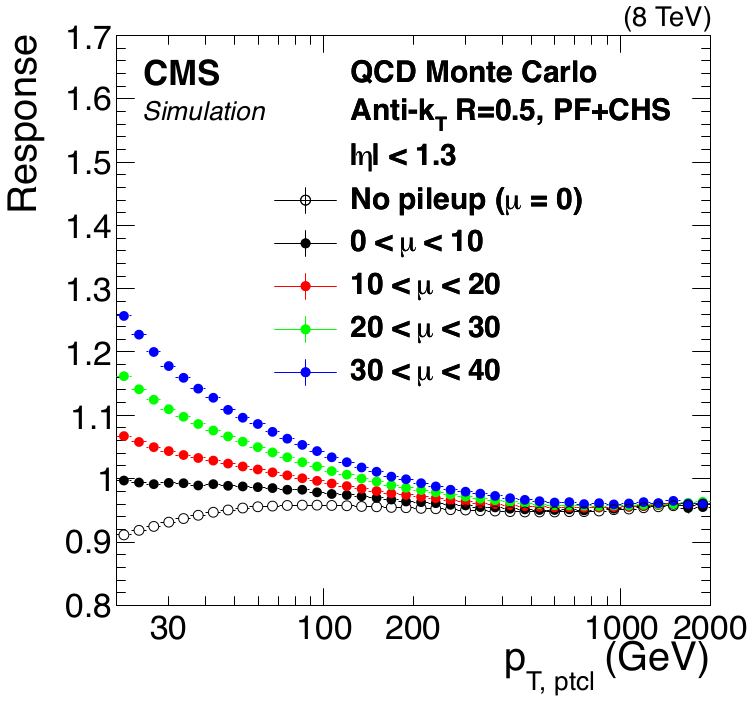
\includegraphics[height = \textheight/2]{\PhDthesisdir/plots_and_images/from_JERC_RunI/response_evolution_1.png}
\hfill
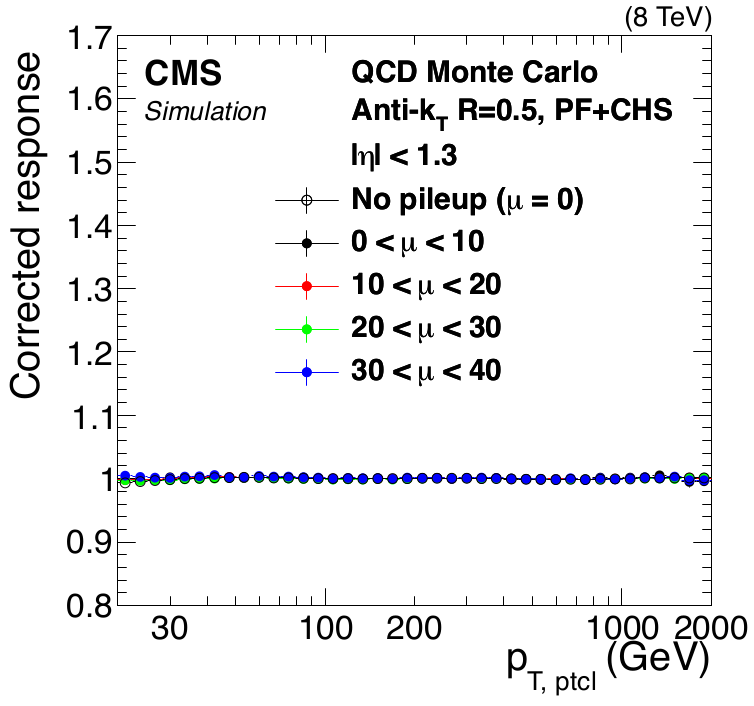
\includegraphics[height = \textheight/2]{\PhDthesisdir/plots_and_images/from_JERC_RunI/response_evolution_3.png}
\end{frame}

\begin{frame}[t]
\addtocounter{framenumber}{-1}
%\transdissolve
\large
\includegraphics[width=\textwidth]{\PhDthesisdir/plots_and_images/from_JERC_RunI/CMS-JME-13-004_Figure_002-FR-TeX-sequential_for_slides/2.tex}

\vfill

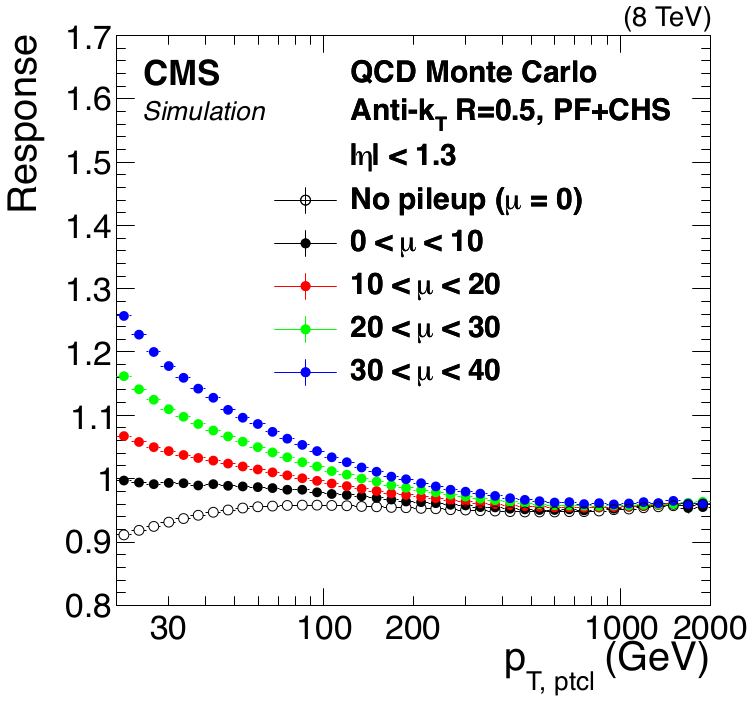
\includegraphics[height = \textheight/2]{\PhDthesisdir/plots_and_images/from_JERC_RunI/response_evolution_1.png}
\hfill
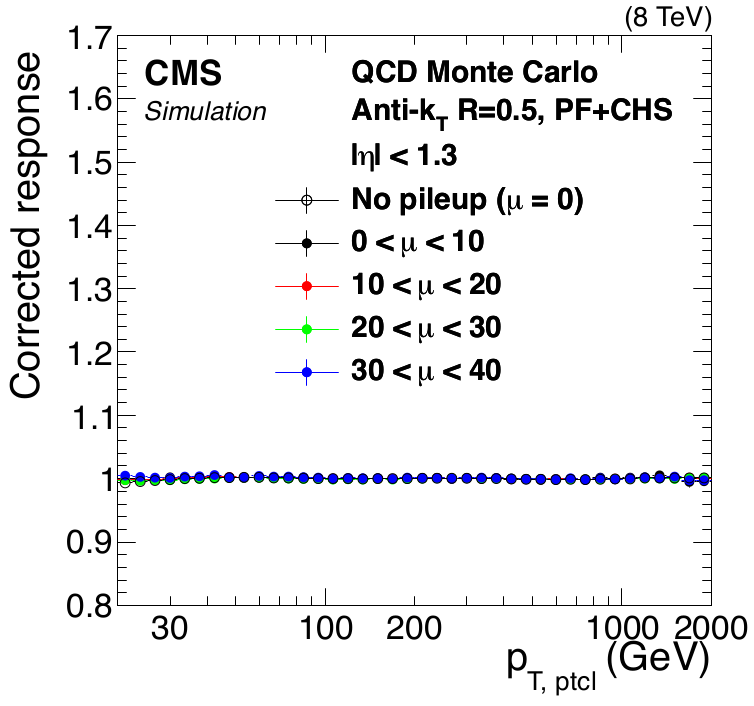
\includegraphics[height = \textheight/2]{\PhDthesisdir/plots_and_images/from_JERC_RunI/response_evolution_3.png}
\end{frame}

\begin{frame}[t]
\addtocounter{framenumber}{-1}
%\transdissolve
\large
\includegraphics[width=\textwidth]{\PhDthesisdir/plots_and_images/from_JERC_RunI/CMS-JME-13-004_Figure_002-FR-TeX-sequential_for_slides/3.tex}

\vfill

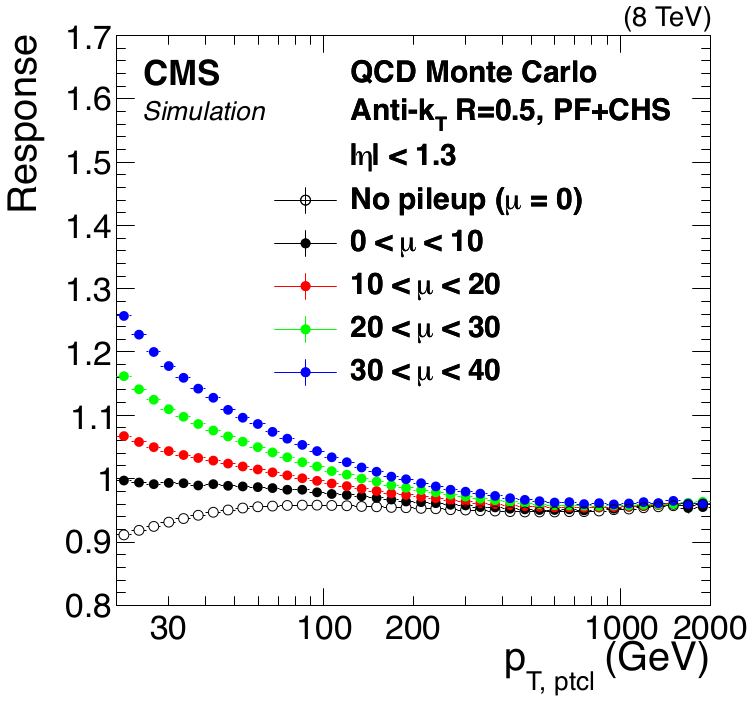
\includegraphics[height = \textheight/2]{\PhDthesisdir/plots_and_images/from_JERC_RunI/response_evolution_1.png}
\hfill
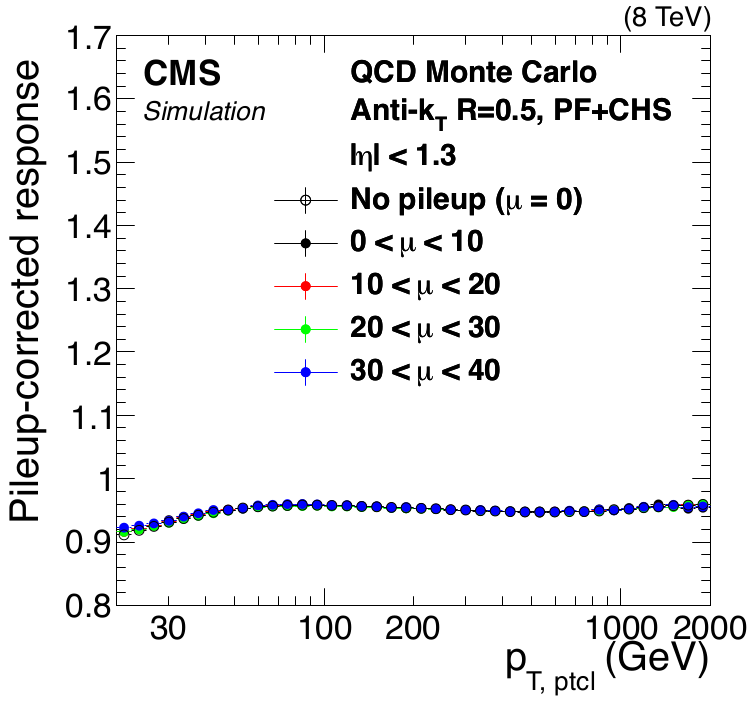
\includegraphics[height = \textheight/2]{\PhDthesisdir/plots_and_images/from_JERC_RunI/response_evolution_2.png}
\hfill
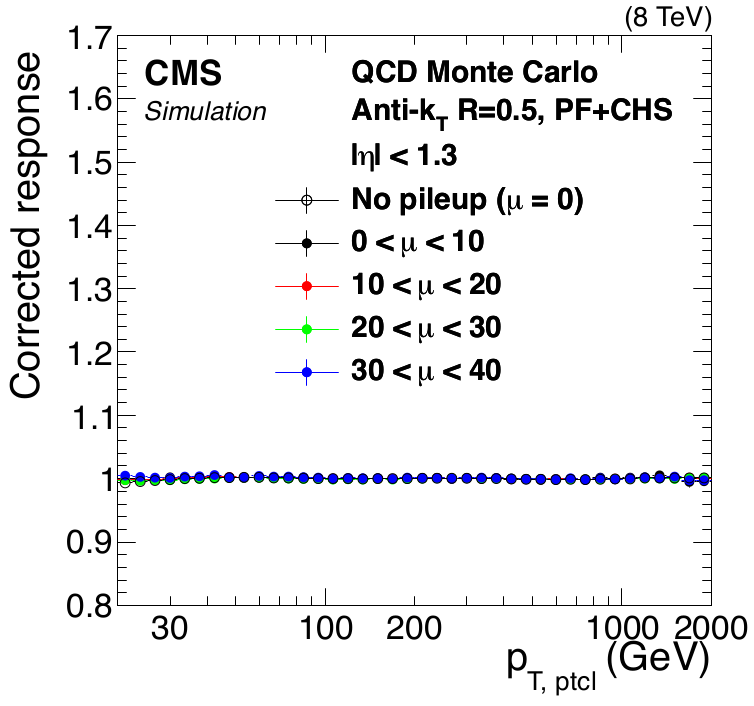
\includegraphics[height = \textheight/2]{\PhDthesisdir/plots_and_images/from_JERC_RunI/response_evolution_3.png}
\end{frame}

\begin{frame}[t]
\addtocounter{framenumber}{-1}
%\transdissolve
\large
\includegraphics[width=\textwidth]{\PhDthesisdir/plots_and_images/from_JERC_RunI/CMS-JME-13-004_Figure_002-FR-TeX-sequential_for_slides/4.tex}

\vfill

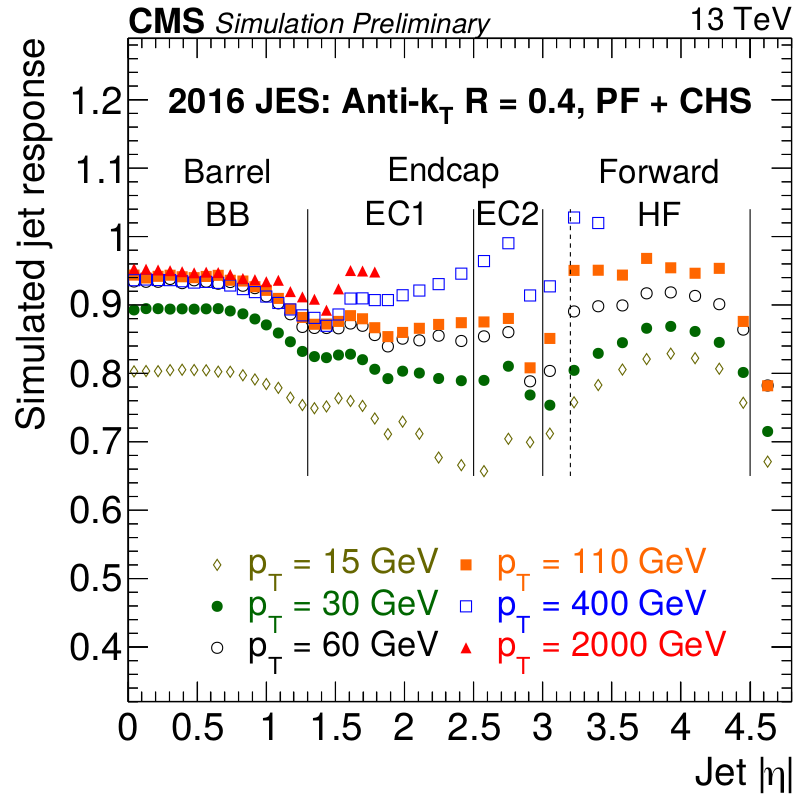
\includegraphics[height = \textheight/2]{\PhDthesisdir/plots_and_images/from_CMS-DP-2020-019/simulated_jet_response_2016.png}
\hfill
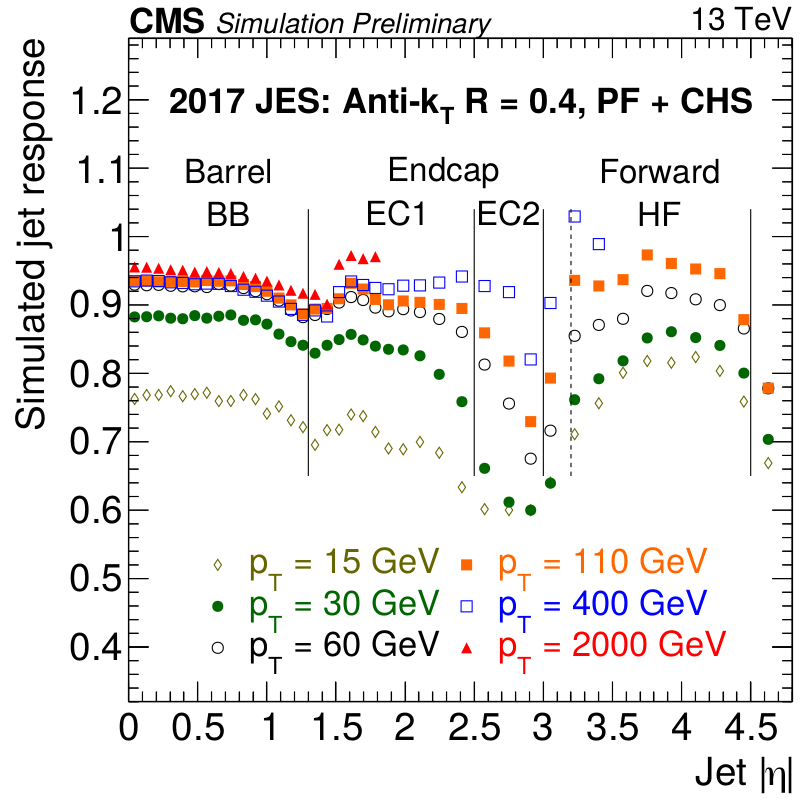
\includegraphics[height = \textheight/2]{\PhDthesisdir/plots_and_images/from_CMS-DP-2020-019/simulated_jet_response_2017.png}
\hfill
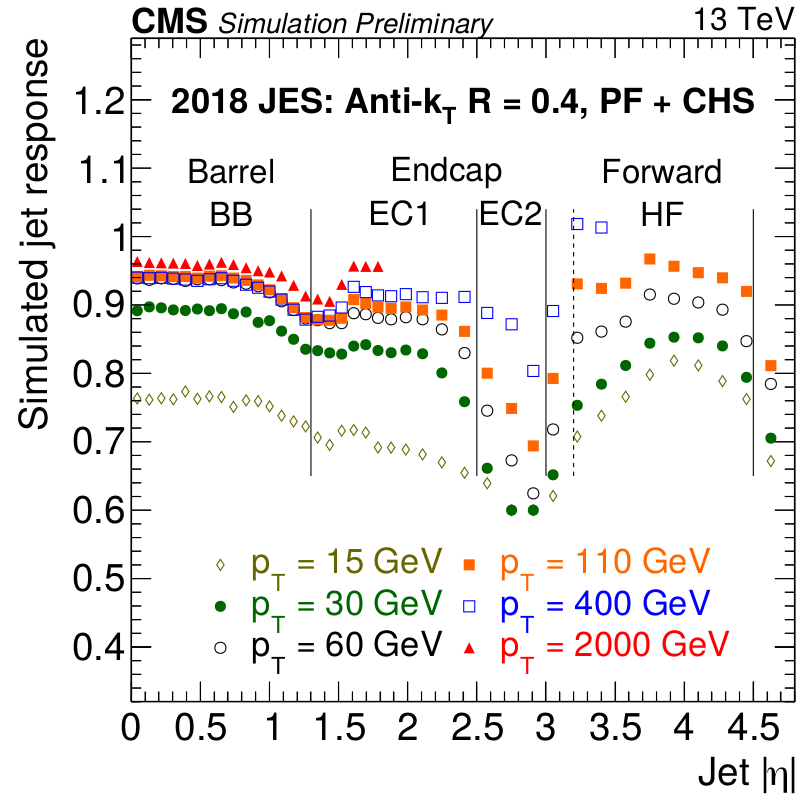
\includegraphics[height = \textheight/2]{\PhDthesisdir/plots_and_images/from_CMS-DP-2020-019/simulated_jet_response_2018.png}
\end{frame}

\begin{frame}[t]
\addtocounter{framenumber}{-1}
%\transdissolve
\large
\includegraphics[width=\textwidth]{\PhDthesisdir/plots_and_images/from_JERC_RunI/CMS-JME-13-004_Figure_002-FR-TeX-sequential_for_slides/5.tex}
\end{frame}

\begin{frame}[t]
\addtocounter{framenumber}{-1}
%\transdissolve
\large
\includegraphics[width=\textwidth]{\PhDthesisdir/plots_and_images/from_JERC_RunI/CMS-JME-13-004_Figure_002-FR-TeX-sequential_for_slides/6.tex}

\vfill

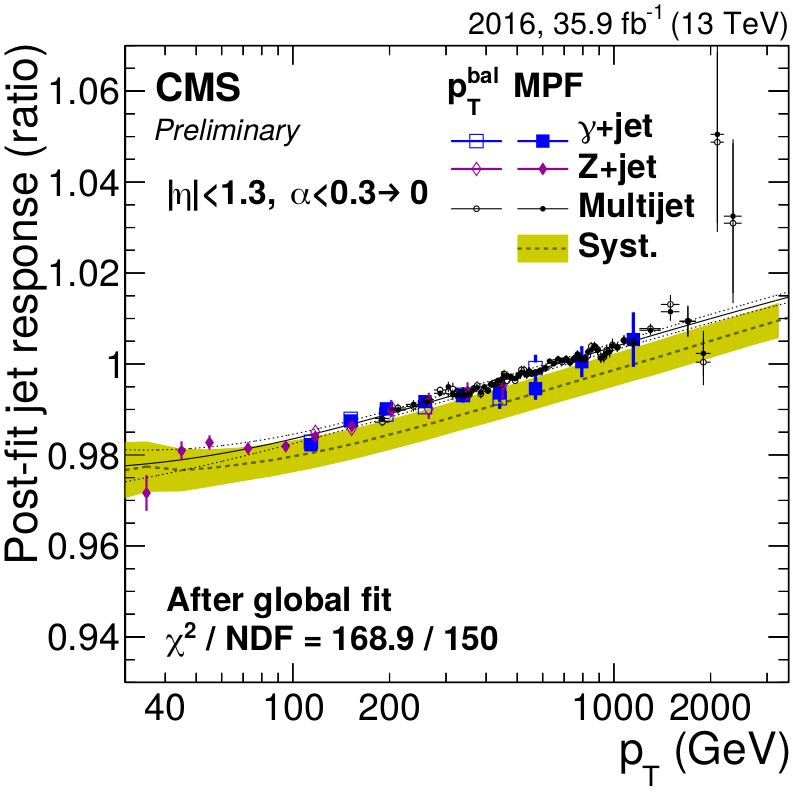
\includegraphics[height = \textheight/2]{\PhDthesisdir/plots_and_images/from_CMS-DP-2020-019/absolute_pT_residual_2016.png}
\hfill
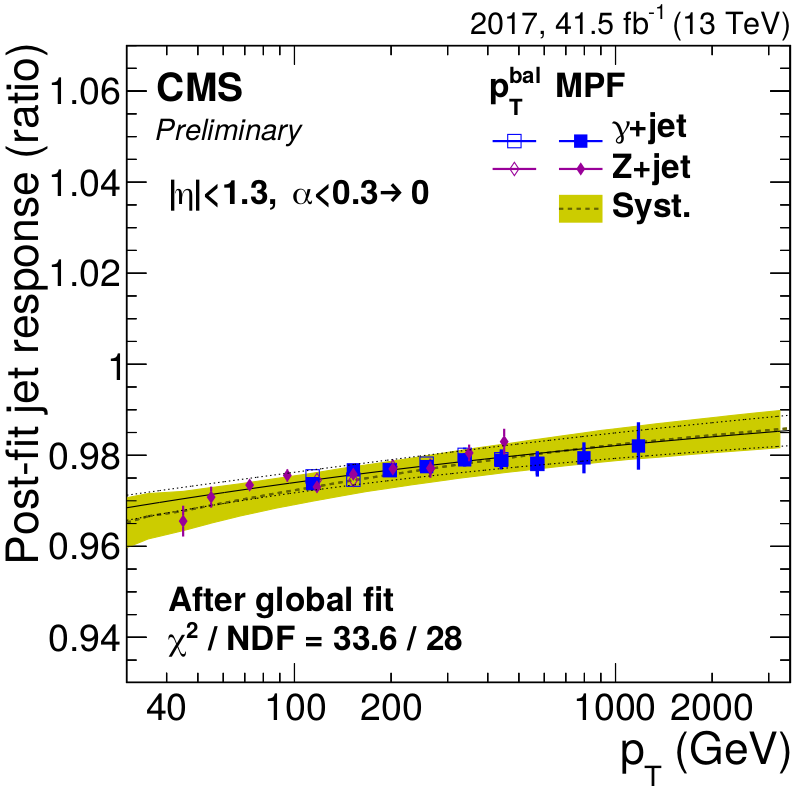
\includegraphics[height = \textheight/2]{\PhDthesisdir/plots_and_images/from_CMS-DP-2020-019/absolute_pT_residual_2017.png}
\hfill
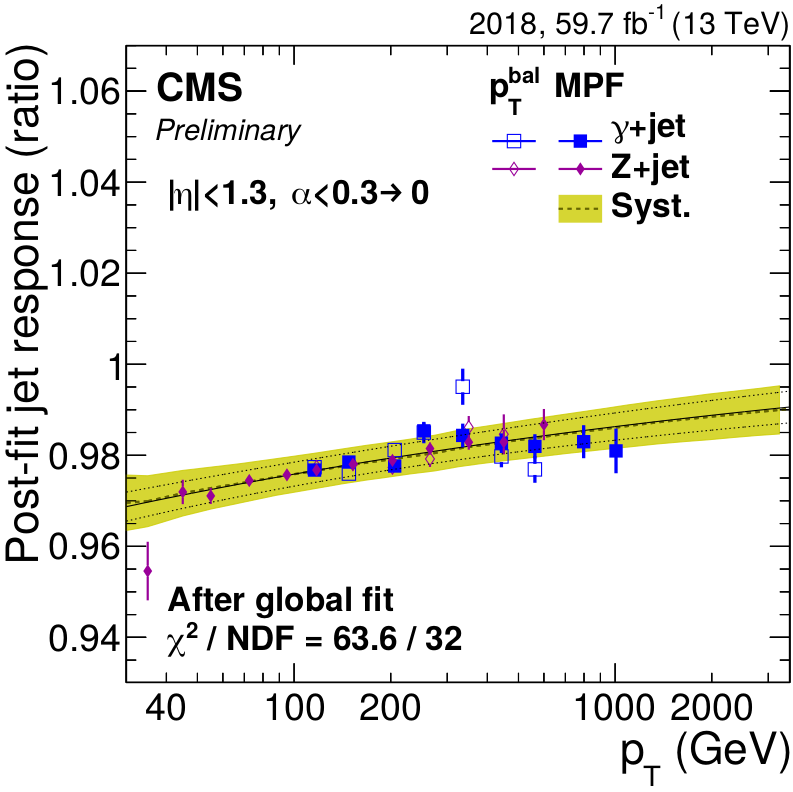
\includegraphics[height = \textheight/2]{\PhDthesisdir/plots_and_images/from_CMS-DP-2020-019/absolute_pT_residual_2018.png}
\end{frame}

\begin{frame}[t]
\addtocounter{framenumber}{-1}
%\transdissolve
\large
\includegraphics[width=\textwidth]{\PhDthesisdir/plots_and_images/from_JERC_RunI/CMS-JME-13-004_Figure_002-FR-TeX.tex}

\vfill

\begin{center}
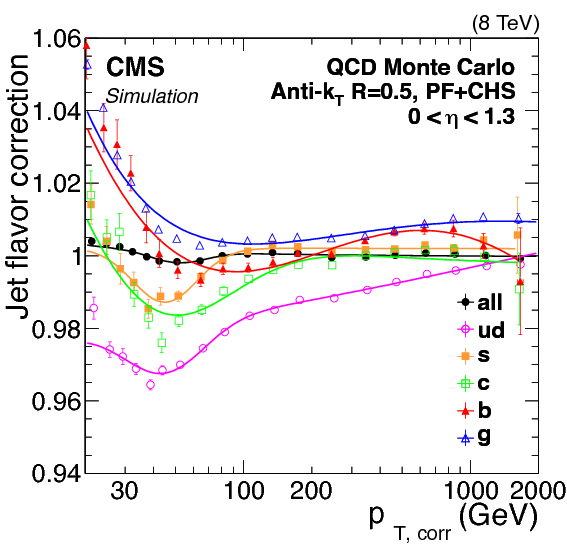
\includegraphics[height = \textheight/2]{\PhDthesisdir/plots_and_images/from_JERC_RunI/Figure_030-a.png}
\end{center}
\end{frame}



\subsection*{Correction résiduelle absolue en \pT\ avec des événements \Gjets}
%\begin{tikzpicture}
\clip (0,0) circle (\HCALrout);

\drawCMS

\printphotondeposit{-135}
\printphoton{-135}


\printbigjetdeposit{9}{45}
\printbigjetnolabel{9}{45}
\printbigjetlabel{9}{35}
\end{tikzpicture}

\begin{frame}
\begin{center}
\includegraphics[width=\graphw,height=\graphh,keepaspectratio]{\PhDthesisdir/plots_and_images/Event_displays/JERC/Gamma_plus_jet.tex}
\end{center}
\end{frame}

\begin{frame}[t]
\vspace{\baselineskip}

~\hfill
\begin{fmffile}{gq_qGamma_S}\fmfstraight
\begin{fmfchar*}(20,20)
  \fmfleft{i1,i2}
  \fmfright{o1,o2}
  \fmf{gluon}{i2,v1}
  \fmf{fermion}{i1,v1,v2,o2}
  \fmf{photon}{v2,o1}
  \fmflabel{\gluon}{i2}
  \fmflabel{\quark}{i1}
  \fmflabel{\quark}{o2}
  \fmflabel{\photon}{o1}
  \fmfdot{v1,v2}
\end{fmfchar*}
\end{fmffile}
\hfill\hfill\hfill
\begin{fmffile}{gq_qGamma_T}\fmfstraight
\begin{fmfchar*}(20,20)
  \fmfleft{i1,i2}
  \fmfright{o1,o2}
  \fmf{gluon}{i2,v2}
  \fmf{fermion}{i1,v1,v2,o2}
  \fmf{photon}{v1,o1}
  \fmflabel{\gluon}{i2}
  \fmflabel{\quark}{i1}
  \fmflabel{\quark}{o2}
  \fmflabel{\photon}{o1}
  \fmfdot{v1,v2}
\end{fmfchar*}
\end{fmffile}
\hfill\hfill\hfill
\begin{fmffile}{qq_gGamma}\fmfstraight
\begin{fmfchar*}(20,20)
  \fmfleft{i1,i2}
  \fmfright{o1,o2}
  \fmf{gluon}{v2,o2}
  \fmf{fermion}{i1,v1,v2,i2}
  \fmf{photon}{v1,o1}
  \fmflabel{\antiquark}{i2}
  \fmflabel{\quark}{i1}
  \fmflabel{\gluon}{o2}
  \fmflabel{\photon}{o1}
  \fmfdot{v1,v2}
\end{fmfchar*}
\end{fmffile}
\hfill~

\pause
\vfill

\begin{equation*}
\vpT_\ptcl^{\photon} + \vpT_\ptcl^\text{jet} = \vec{0}
\Rightarrow
\pT_\ptcl^{\photon} = \pT_\ptcl^\text{jet}
\end{equation*}
\pause
\begin{equation*}
R
= \frac{\pT_\reco^\text{jet}}{\pT_\ptcl^\text{jet}}
= \frac{\pT_\reco^\text{jet}}{\pT_\ptcl^{\photon}}
\simeq \frac{\pT_\reco^\text{jet}}{\pT_\reco^{\photon}}
\end{equation*}
\pause
\begin{equation*}
\Rbal = \frac{\pT_\reco^\text{jet}}{\pT^{\photon}}
\end{equation*}

%\manip Only 2 \og particles \fg{} (physics objects) in final state:
%\begin{itemize}
%\item photon (well known);
%\item jet (to calibrate).
%\end{itemize}
%\manip No neutrino $\Rightarrow$ no real \MET.
\end{frame}

%\begin{frame}
\transduration{0}
\begin{center}
\includegraphics[width=\graphw,height=\graphh,keepaspectratio]{/home/torterotot/Documents/PhD-Thesis/plots_and_images/Event_displays/JERC/slides_anims/Gamma_plus_2jets/1.tex}
\end{center}
\end{frame}

\begin{frame}
\addtocounter{framenumber}{-1}
\transboxout
\transduration{0}
\begin{center}
\includegraphics[width=\graphw,height=\graphh,keepaspectratio]{/home/torterotot/Documents/PhD-Thesis/plots_and_images/Event_displays/JERC/slides_anims/Gamma_plus_2jets/2.tex}
\end{center}
\end{frame}

\begin{frame}
\addtocounter{framenumber}{-1}
\transdissolve
\begin{center}
\includegraphics[width=\graphw,height=\graphh,keepaspectratio]{\PhDthesisdir/plots_and_images/Event_displays/JERC/Gamma_plus_2jets.tex}
\end{center}
\end{frame}
\begin{frame}
\begin{center}
\includegraphics[width=\graphw,height=\graphh,keepaspectratio]{\PhDthesisdir/plots_and_images/Event_displays/JERC/Gamma_plus_2jets.tex}
\end{center}
\end{frame}

\begin{frame}[t]
\vspace{\baselineskip}

~\hfill
\begin{fmffile}{gq_qGamma_T}\fmfstraight
\begin{fmfchar*}(20,20)
  \fmfleft{i1,i2}
  \fmfright{o1,o2}
  \fmf{gluon}{i2,v2}
  \fmf{fermion}{i1,v1,v2,o2}
  \fmf{photon}{v1,o1}
  \fmflabel{\gluon}{i2}
  \fmflabel{\quark}{i1}
  \fmflabel{\quark}{o2}
  \fmflabel{\photon}{o1}
  \fmfdot{v1,v2}
\end{fmfchar*}
\end{fmffile}
\hfill~

\pause
\vfill

~\hfill
\begin{fmffile}{gq_qGamma_S-ISR_2jets}\fmfstraight
\begin{fmfchar*}(20,20)
  \fmfleft{i1,i2}
  \fmfright{o0,o1,o2}
  \fmf{gluon}{i2,v1}
  \fmf{phantom}{i1,v1}
  \fmf{phantom, tension=2}{v1,v2}
  \fmf{phantom}{v2,o2}
  \fmf{phantom}{v2,o0}
  \fmflabel{\gluon}{i2}
  \fmflabel{\quark}{i1}
  \fmflabel{\quark}{o2}
  \fmflabel{\photon}{o1}
  \fmfdot{v1,v2}
  \fmffreeze
  \fmf{fermion}{i1,v3,v1,v2,o2}
  \fmffreeze
  \fmf{photon}{v2,o1}
  \fmf{gluon}{v3,o0}
  \fmflabel{\gluon}{o0}
  \fmfdot{v3}
\end{fmfchar*}
\end{fmffile}
\hfill\hfill\hfill
\begin{fmffile}{gq_qGamma_S-ISR_2photons}\fmfstraight
\begin{fmfchar*}(20,20)
  \fmfleft{i1,i2}
  \fmfright{o0,o1,o2}
  \fmf{gluon}{i2,v1}
  \fmf{phantom}{i1,v1}
  \fmf{phantom, tension=2}{v1,v2}
  \fmf{phantom}{v2,o2}
  \fmf{phantom}{v2,o0}
  \fmflabel{\gluon}{i2}
  \fmflabel{\quark}{i1}
  \fmflabel{\quark}{o2}
  \fmflabel{\photon}{o1}
  \fmfdot{v1,v2}
  \fmffreeze
  \fmf{fermion}{i1,v3,v1,v2,o2}
  \fmffreeze
  \fmf{photon}{v2,o1}
  \fmf{photon}{v3,o0}
  \fmflabel{\photon}{o0}
  \fmfdot{v3}
\end{fmfchar*}
\end{fmffile}
\hfill\hfill\hfill
\begin{fmffile}{gq_qGamma_S-FSR_2jets}\fmfstraight
\begin{fmfchar*}(20,20)
  \fmfleft{i1,i2}
  \fmfright{o1,o0,o2}
  \fmf{gluon}{i2,v1}
  \fmf{phantom}{i1,v1}
  \fmf{phantom, tension=2}{v1,v2}
  \fmf{phantom}{v2,o2}
  \fmf{photon}{v2,o1}
  \fmflabel{\gluon}{i2}
  \fmflabel{\quark}{i1}
  \fmflabel{\quark}{o2}
  \fmflabel{\photon}{o1}
  \fmfdot{v1,v2}
  \fmffreeze
  \fmf{fermion}{i1,v1,v2,v3,o2}
  \fmffreeze
  \fmf{gluon}{v3,o0}
  \fmflabel{\gluon}{o0}
  \fmfdot{v3}
\end{fmfchar*}
\end{fmffile}
\hfill\hfill\hfill
\begin{fmffile}{gq_qGamma_S-FSR_2photons}\fmfstraight
\begin{fmfchar*}(20,20)
  \fmfleft{i1,i2}
  \fmfright{o1,o0,o2}
  \fmf{gluon}{i2,v1}
  \fmf{phantom}{i1,v1,v2,o2}
  \fmf{photon}{v2,o1}
  \fmflabel{\gluon}{i2}
  \fmflabel{\quark}{i1}
  \fmflabel{\quark}{o2}
  \fmflabel{\photon}{o1}
  \fmfdot{v1,v2}
  \fmffreeze
  \fmf{fermion}{i1,v1,v2,v3,o2}
  \fmffreeze
  \fmf{photon}{v3,o0}
  \fmflabel{\photon}{o0}
  \fmfdot{v3}
\end{fmfchar*}
\end{fmffile}
\hfill~

\end{frame}

\begin{frame}
\begin{minipage}[t]{.45\textwidth}
\begin{equation*}
\Rbal = \frac{\pT_\reco^\text{jet 1}}{\pT^{\photon}}
\end{equation*}
\end{minipage}
\hfill
\begin{minipage}[t]{.45\textwidth}
\begin{equation*}
\alpha = \frac{\pT_\reco^\text{jet 2}}{\pT^{\photon}}
\end{equation*}
\end{minipage}
\end{frame}

\begin{frame}

\begin{equation*}
\vpT^\photon_\ptcl + \vpT^\text{recul}_\ptcl = \vec{0}
\end{equation*}

\pause
\vfill


\begin{equation*}
\vpT^\photon_\reco + \underbrace{\RMPF \vpT^\text{recul}_\ptcl}_{\vpT^\text{recul}_\reco} = -\vMET
\Rightarrow
\boxed{\RMPF = 1 + \frac{\vpT^\photon\cdot\vMET}{\abs{\vpT^\photon}^2}}
\end{equation*}
\end{frame}
\begin{frame}
\frametitle{$\photon+\text{jet}$ events: jet calibration, balancing method}
\manip The physics of the events gives
\begin{equation*}
\vpT^\photon_\ptcl + \vpT^\text{jet}_\ptcl = \vec{0} \Rightarrow \boxed{{\pT}^\photon_\ptcl = {\pT}^\text{jet}_\ptcl}
\end{equation*}

\pause
\vfill

\manip For the reconstructed objects, the balancing response is then defined as
\begin{equation*}
\vpT^\photon_\reco + \underbrace{\Rbal \vpT^\text{jet}_\ptcl}_{\vpT^\text{jet}_\reco} = \vec{0}
\Rightarrow
\boxed{\Rbal = \frac{{\pT}^\text{jet}_\reco}{\pT^\photon}}
\end{equation*}
\begin{equation*}
\text{because }
\pT^\photon_\ptcl\simeq\pT^\photon_\reco
=\pT^\photon
\mend
\end{equation*}
\end{frame}

\begin{frame}
\frametitle{$\photon+\text{jet}$ events: world is not perfect}
\begin{center}
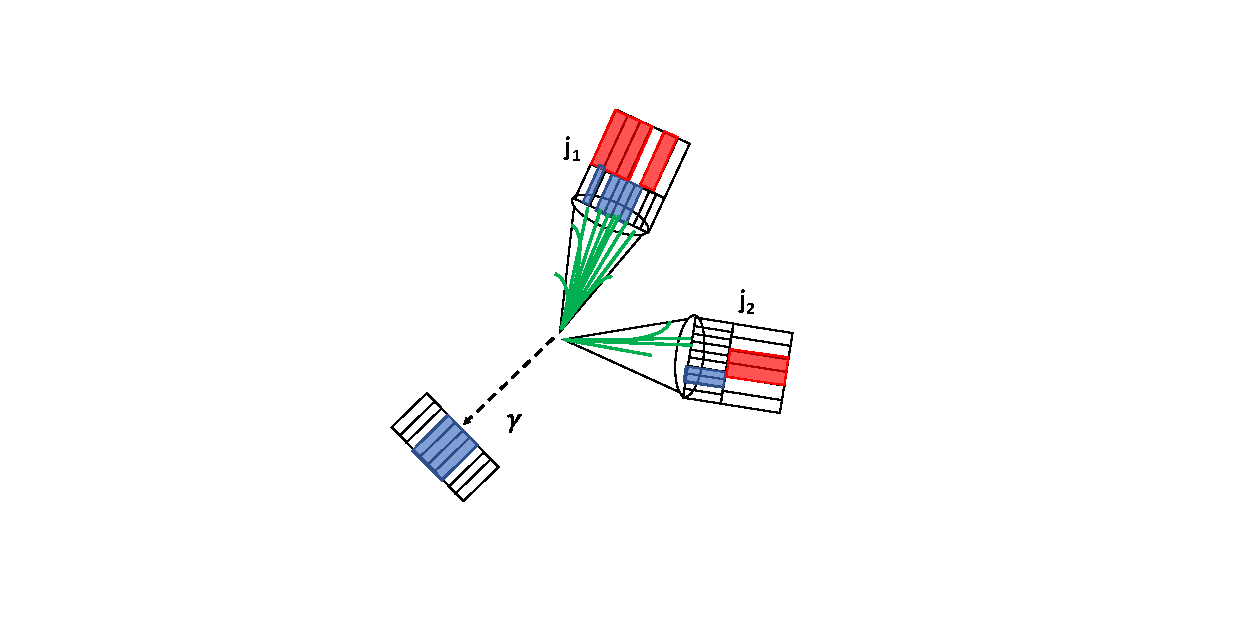
\includegraphics[width=\graphw,height=\graphh,keepaspectratio, trim = 5.5cm 2cm 7.5cm 1.75cm, clip]{\PhDthesisdir/tex/slides/JERC/JEC_Principe/Gamma_plus_two_jets.pdf}
\end{center}
\end{frame}

\begin{frame}
\frametitle{$\photon+\text{jet}$ events: world is not perfect}
\manip Imbalance due to the presence of additionnal jets.
\pause
\manip Use the jet with higher \pT: $\displaystyle \boxed{\Rbal = \frac{{\pT}^\text{1\up{st}jet}_\reco}{\pT^\photon}}$.
\pause
\manip To avoid correction on additonnal jets: define $\displaystyle \boxed{\alpha = \frac{{\pT}^\text{2\up{nd}jet}_\reco}{\pT^\photon}}$ and extrapolate to $\alpha=0$.
\end{frame}

\begin{frame}
\frametitle{$\photon+\text{jet}$ events: jet calibration, MPF method}
\manip Considering balance between photon and \emph{all other particles},
\begin{equation*}
\vpT^\photon_\ptcl + \vpT^\text{recoil}_\ptcl = \vec{0}
\end{equation*}

\pause
\vfill

\manip For the reconstructed objects, the MPF response is then defined as
\begin{equation*}
\vpT^\photon_\reco + \underbrace{\RMPF \vpT^\text{recoil}_\ptcl}_{\vpT^\text{recoil}_\reco} = -\vMET
\Rightarrow
\boxed{\RMPF = 1 + \frac{\vpT^\photon\cdot\vMET}{\abs{\vpT^\photon}^2}}
\end{equation*}
\end{frame}
\begin{frame}
\frametitle{Run 2018 ABCD responses, $\alpha=\num{0.15}$, $\eta\in [\num{0},\num{1.3}]$}
\begin{minipage}{.45\textwidth}
\begin{figure}
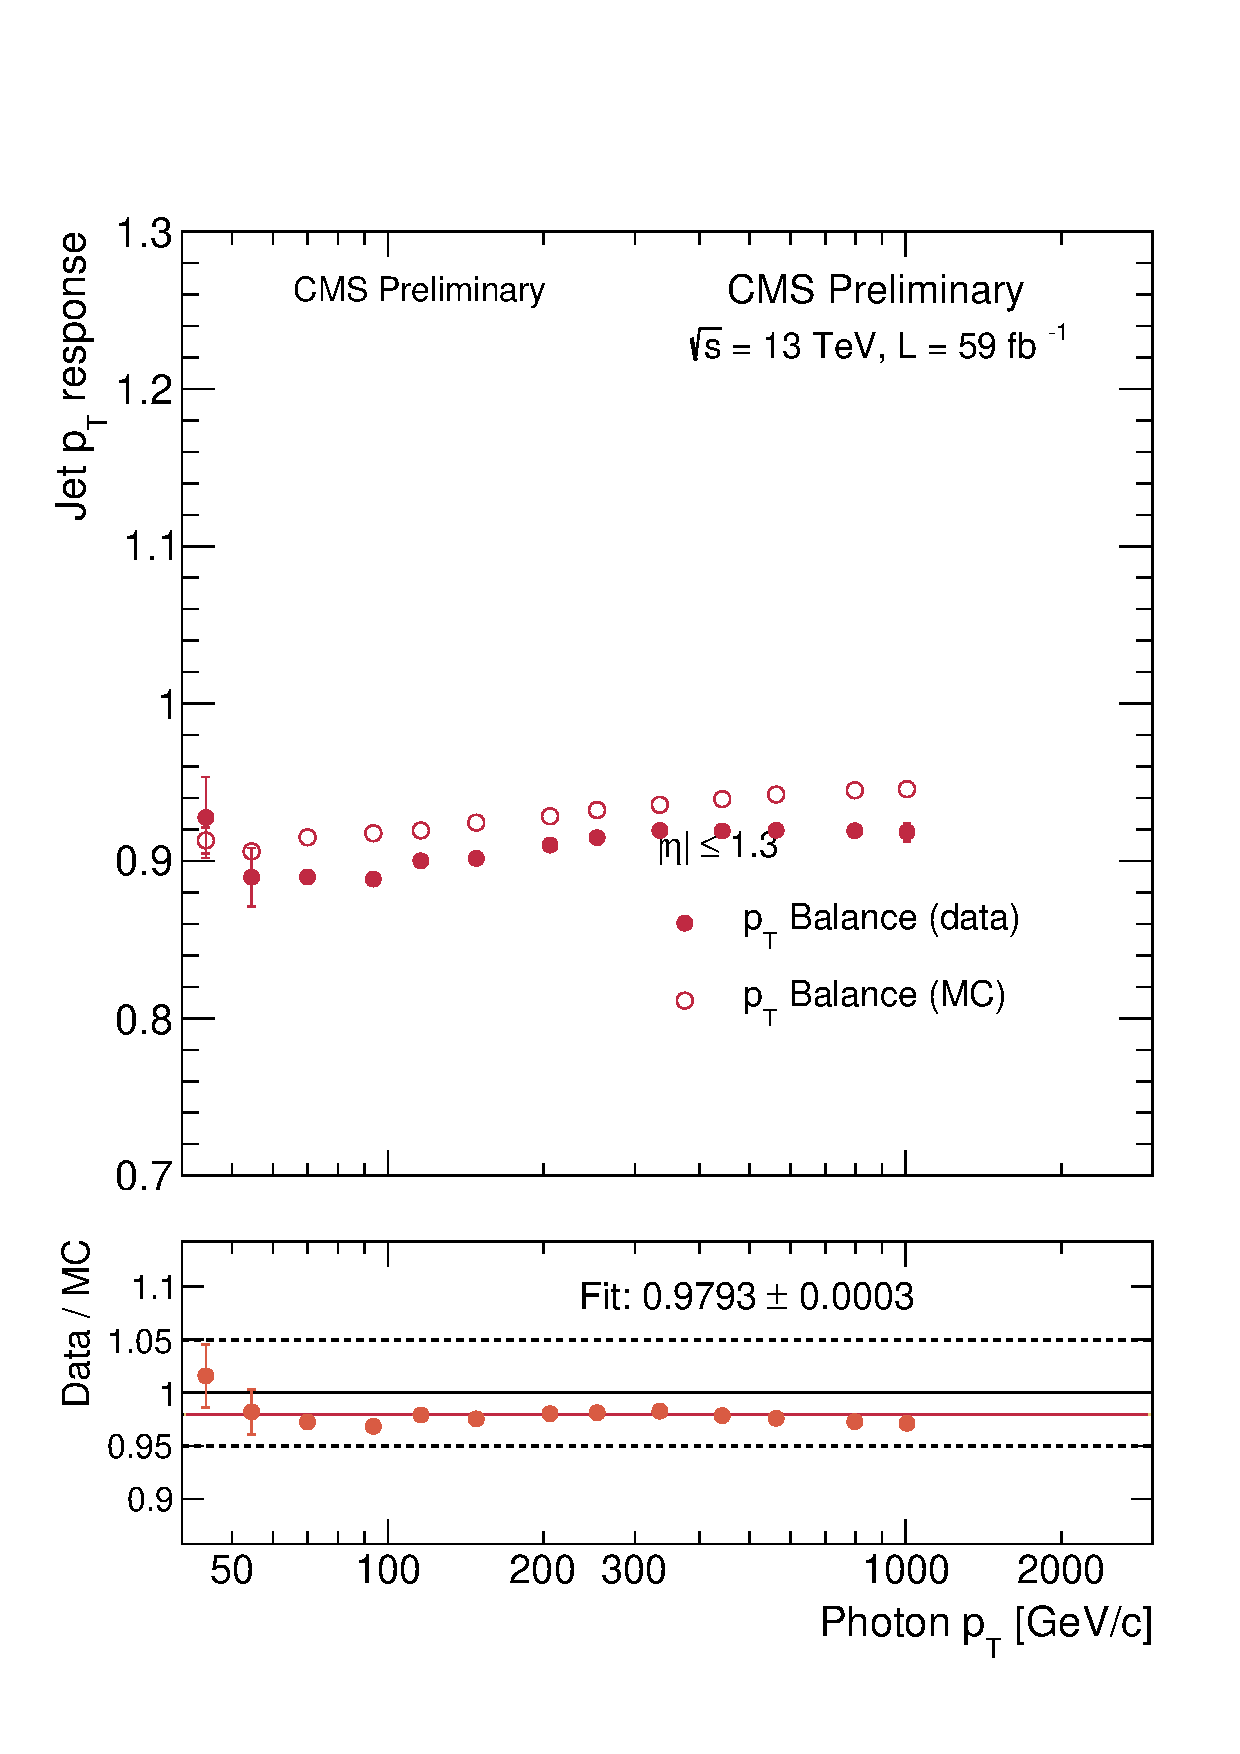
\includegraphics[width=.9\linewidth]{\PhDthesisdir/contents/chapter-JERC/plots/2019-07-25/only_L2Res/Run2018ABCD/alpha_0_15/response_eta0013_balancing.pdf}
\caption{Balancing}
\end{figure}
\end{minipage}
\hfill
\begin{minipage}{.45\textwidth}
\begin{figure}
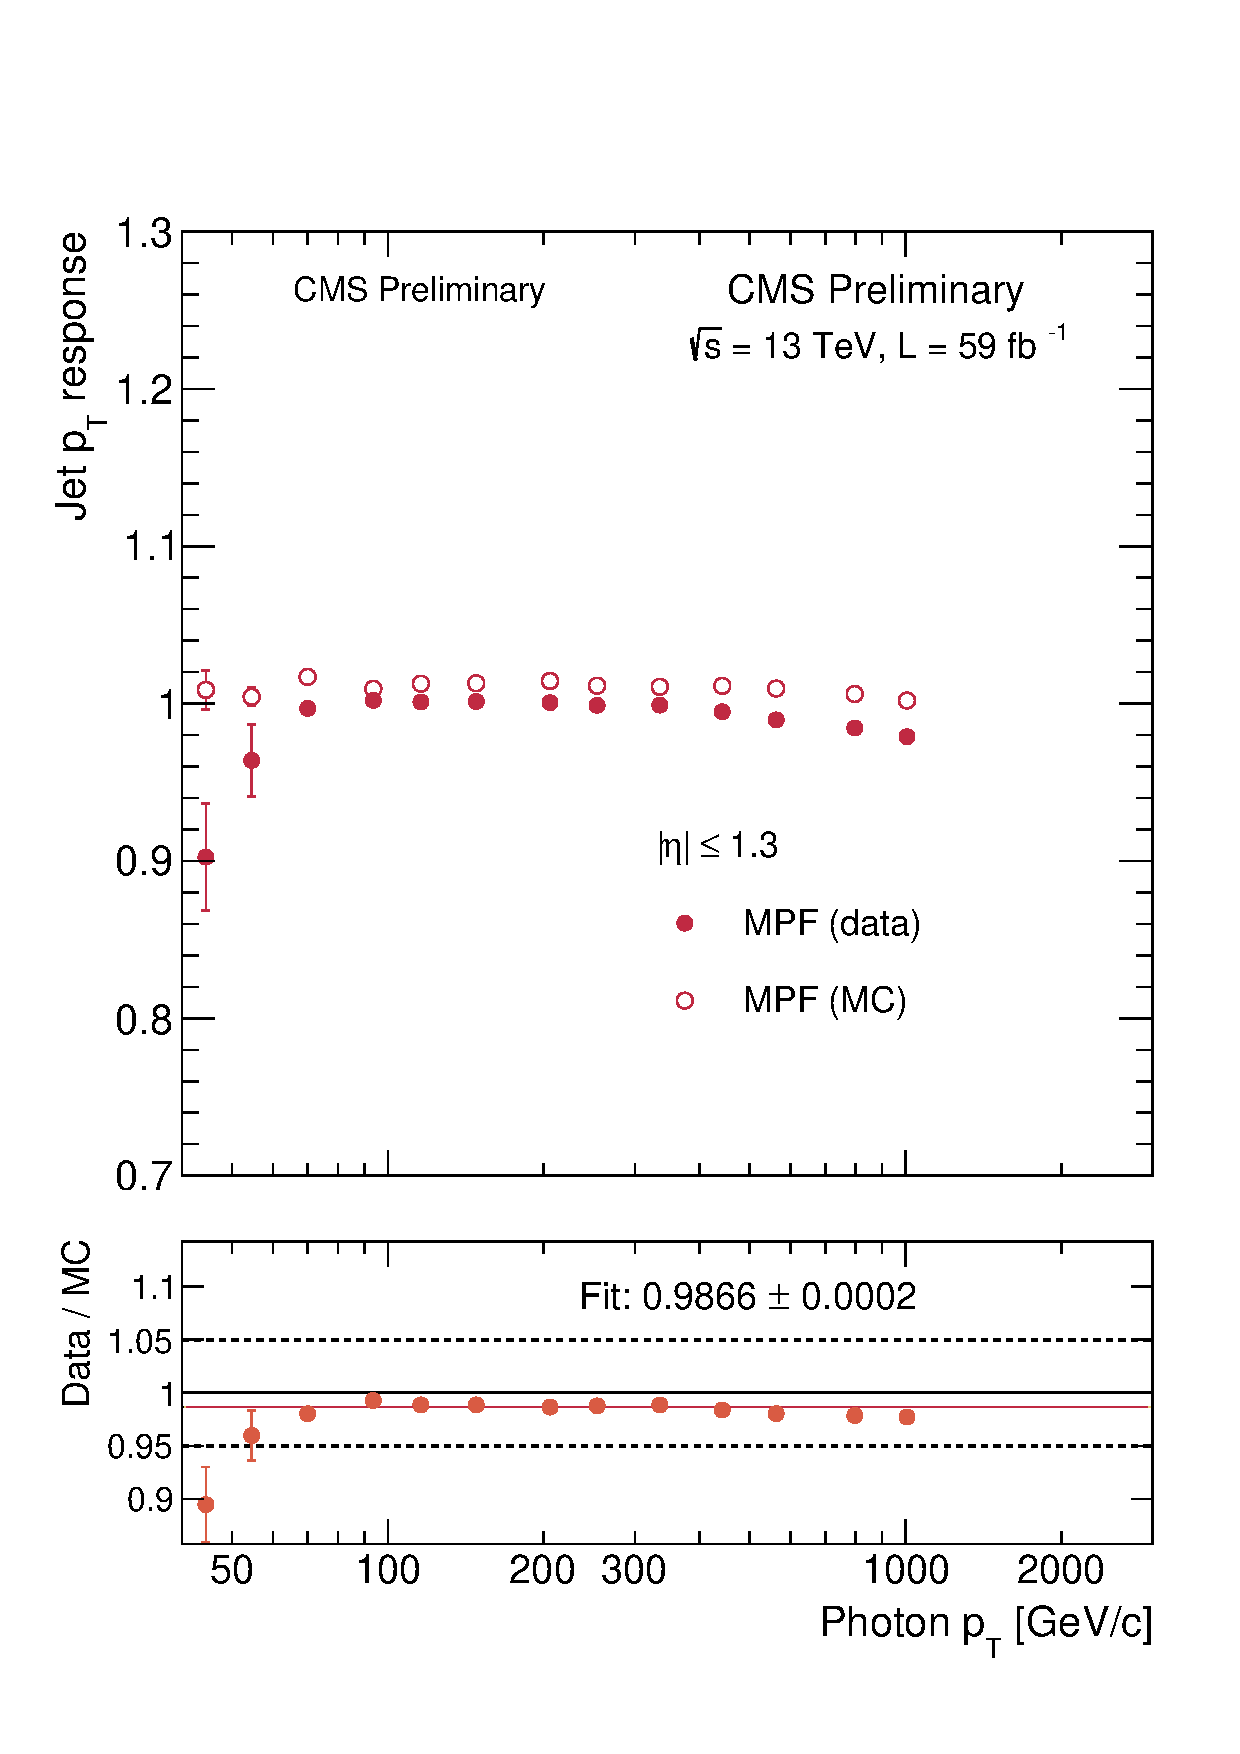
\includegraphics[width=.9\linewidth]{\PhDthesisdir/contents/chapter-JERC/plots/2019-07-25/only_L2Res/Run2018ABCD/alpha_0_15/response_eta0013_mpf.pdf}
\caption{MPF}
\end{figure}
\end{minipage}
\end{frame}

\begin{frame}
\frametitle{Run 2018 ABCD responses, extrapolation, $\pT\in [\num{175},\num{230}]\SI{}{\GeV}$, $\eta\in [\num{0},\num{1.3}]$}
\begin{minipage}{.45\textwidth}
\begin{figure}
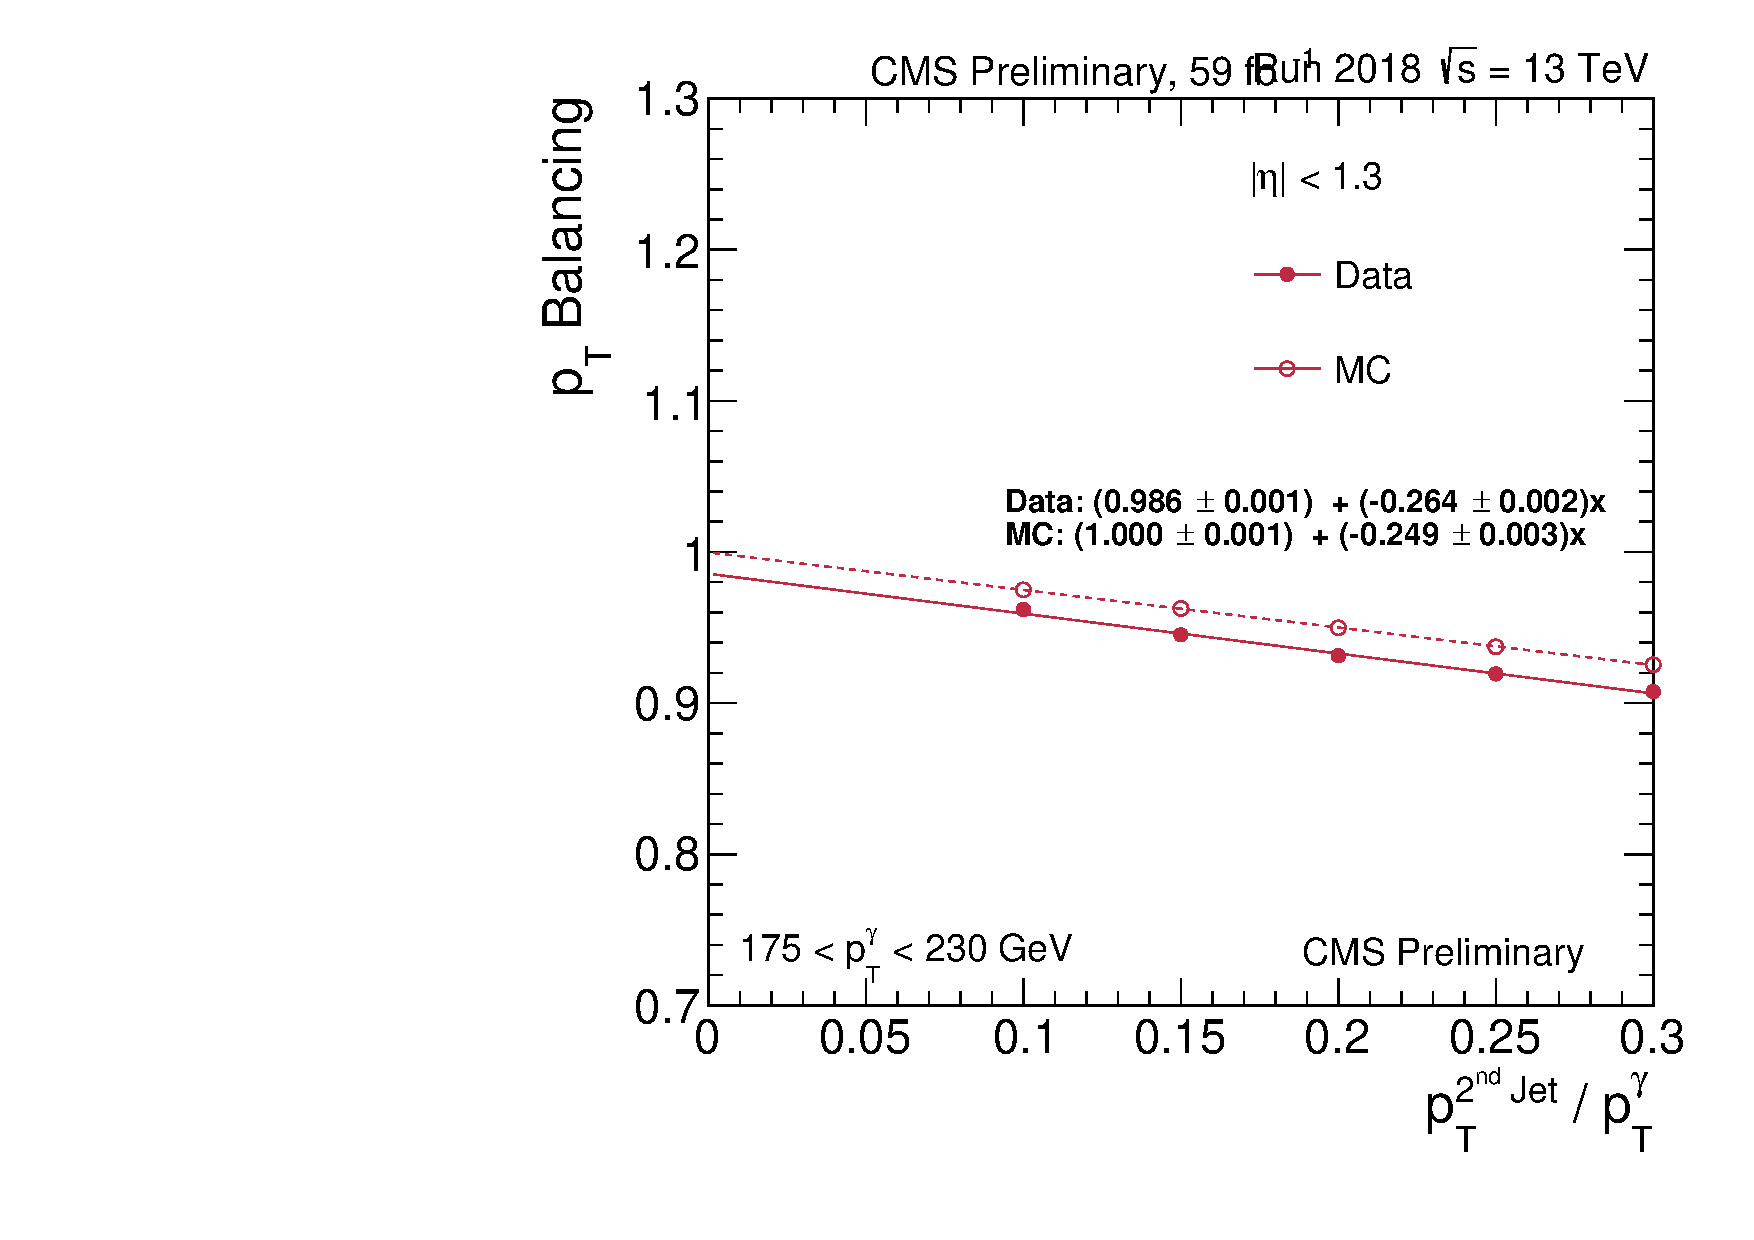
\includegraphics[width=.9\linewidth]{\PhDthesisdir/contents/chapter-JERC/plots/2019-07-25/only_L2Res/Run2018ABCD/extrapolation/response_eta0013_ptPhot_175_230.pdf}
\caption{Balancing}
\end{figure}
\end{minipage}
\hfill
\begin{minipage}{.45\textwidth}
\begin{figure}
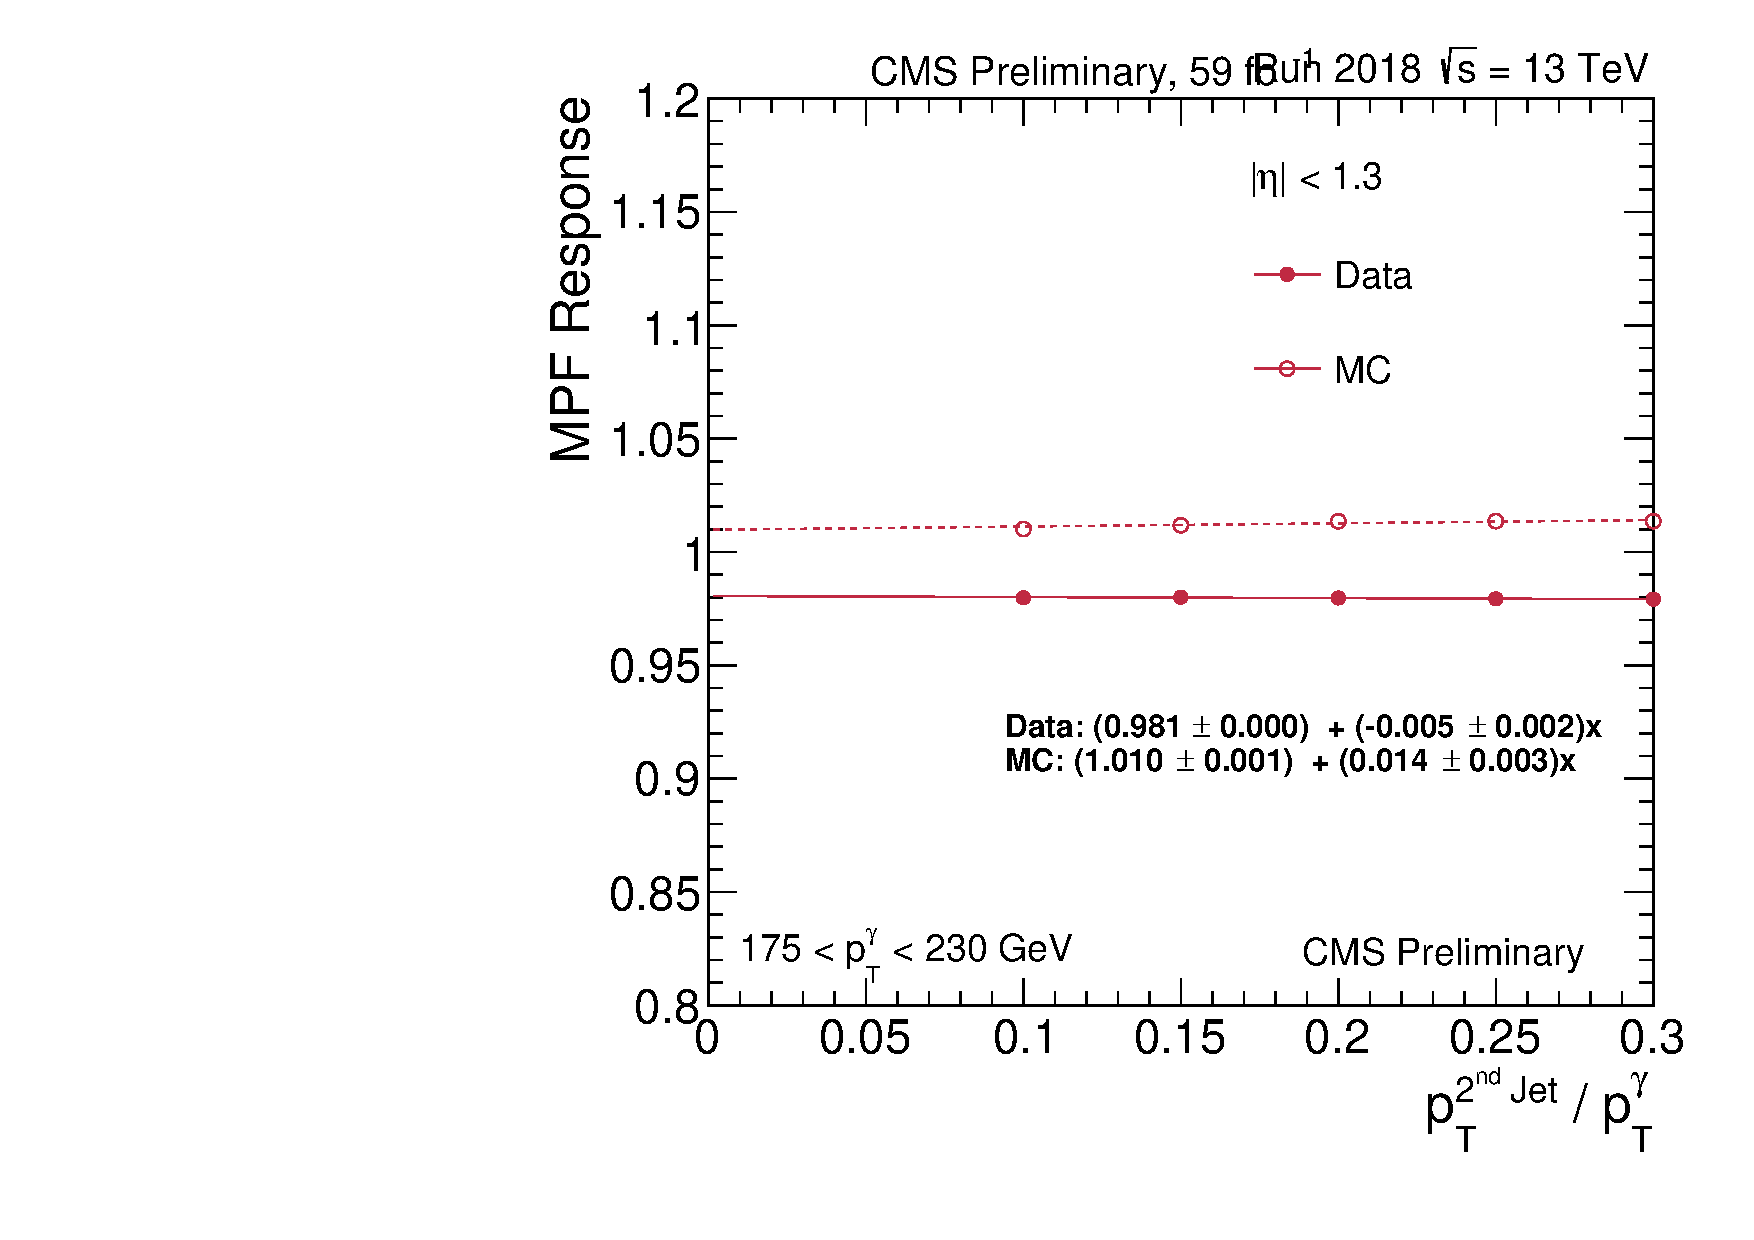
\includegraphics[width=.9\linewidth]{\PhDthesisdir/contents/chapter-JERC/plots/2019-07-25/only_L2Res/Run2018ABCD/extrapolation/responseMPF_eta0013_ptPhot_175_230.pdf}
\caption{MPF}
\end{figure}
\end{minipage}
\end{frame}

\begin{frame}
\frametitle{Run 2018 ABCD responses, extrapolated, $\eta\in [\num{0},\num{1.3}]$}
\begin{minipage}{.45\textwidth}
\begin{figure}
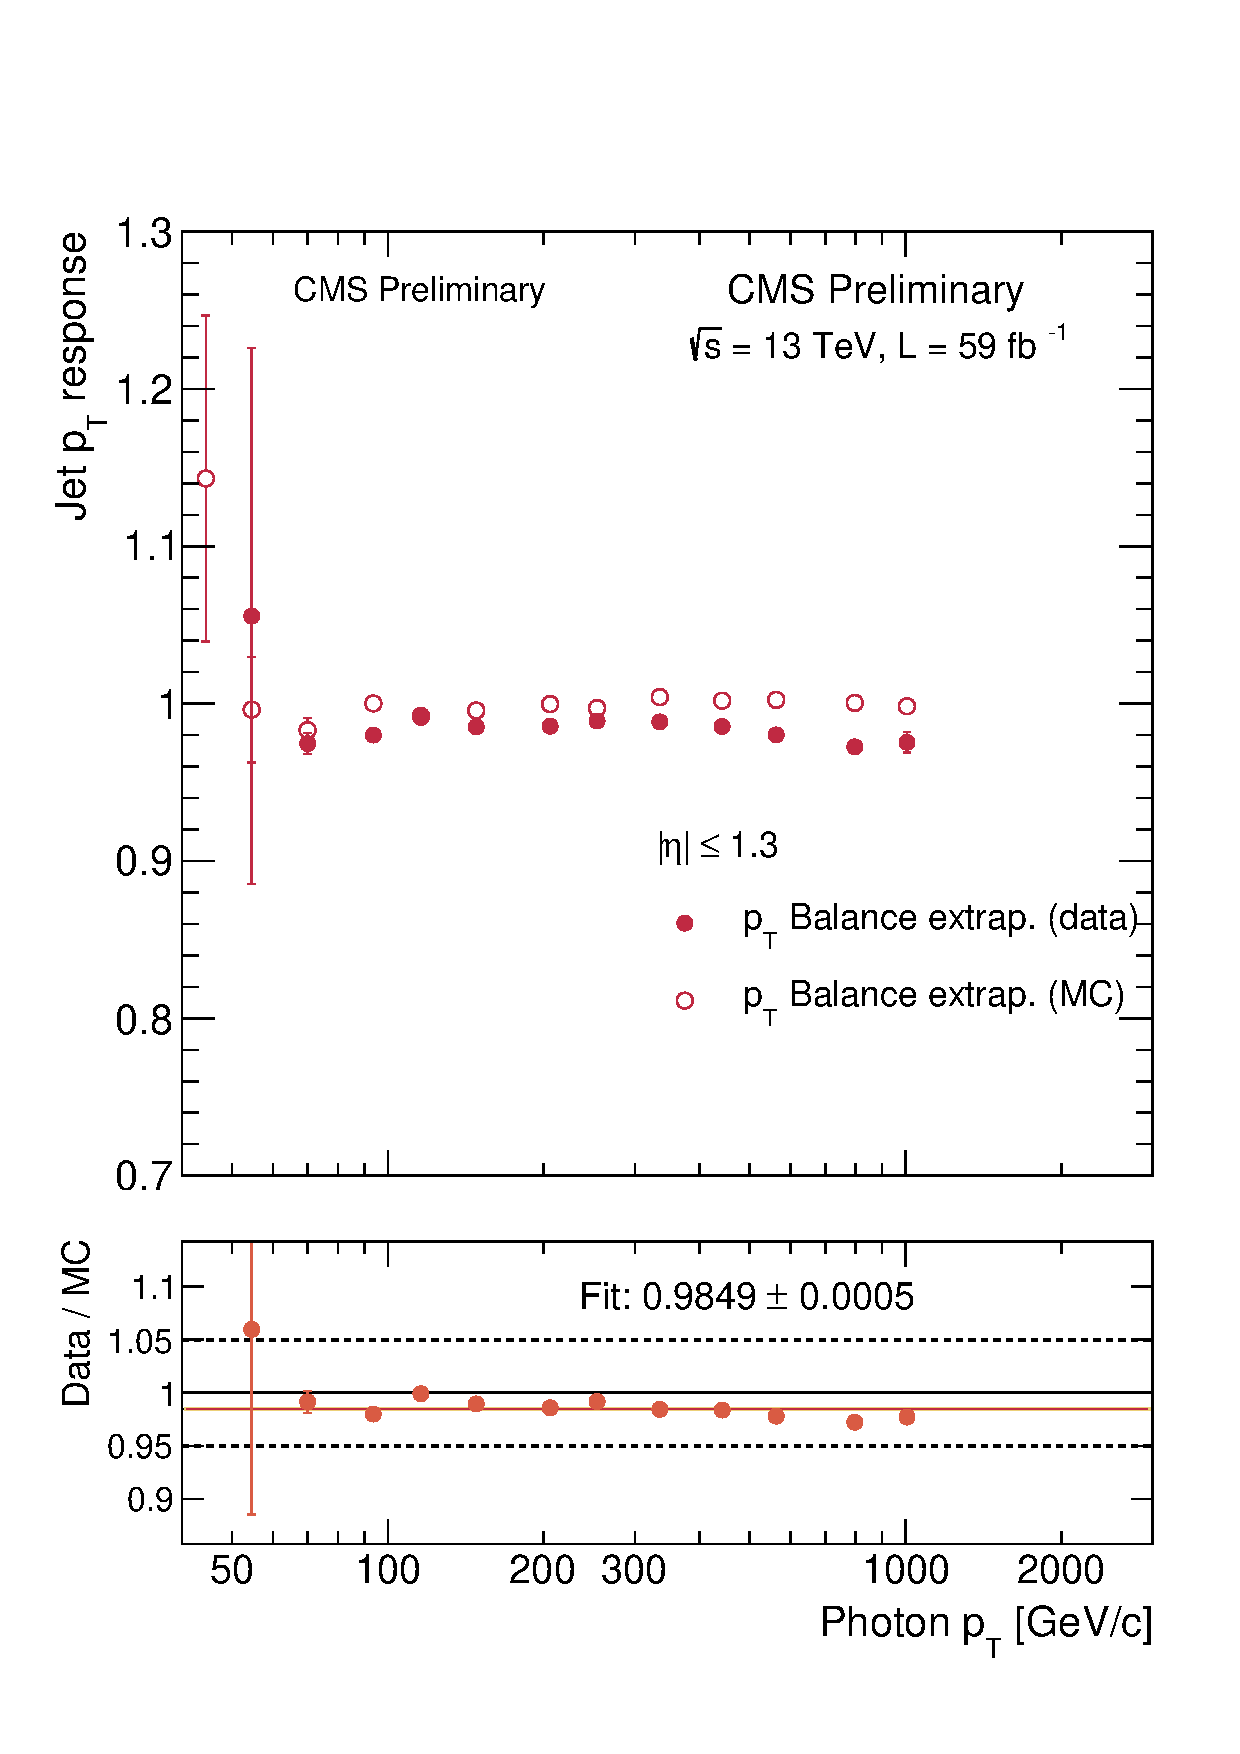
\includegraphics[width=.9\linewidth]{\PhDthesisdir/contents/chapter-JERC/plots/2019-07-25/only_L2Res/Run2018ABCD/extrapolated/response_eta0013_balancing_extrap.pdf}
\caption{Balancing}
\end{figure}
\end{minipage}
\hfill
\begin{minipage}{.45\textwidth}
\begin{figure}
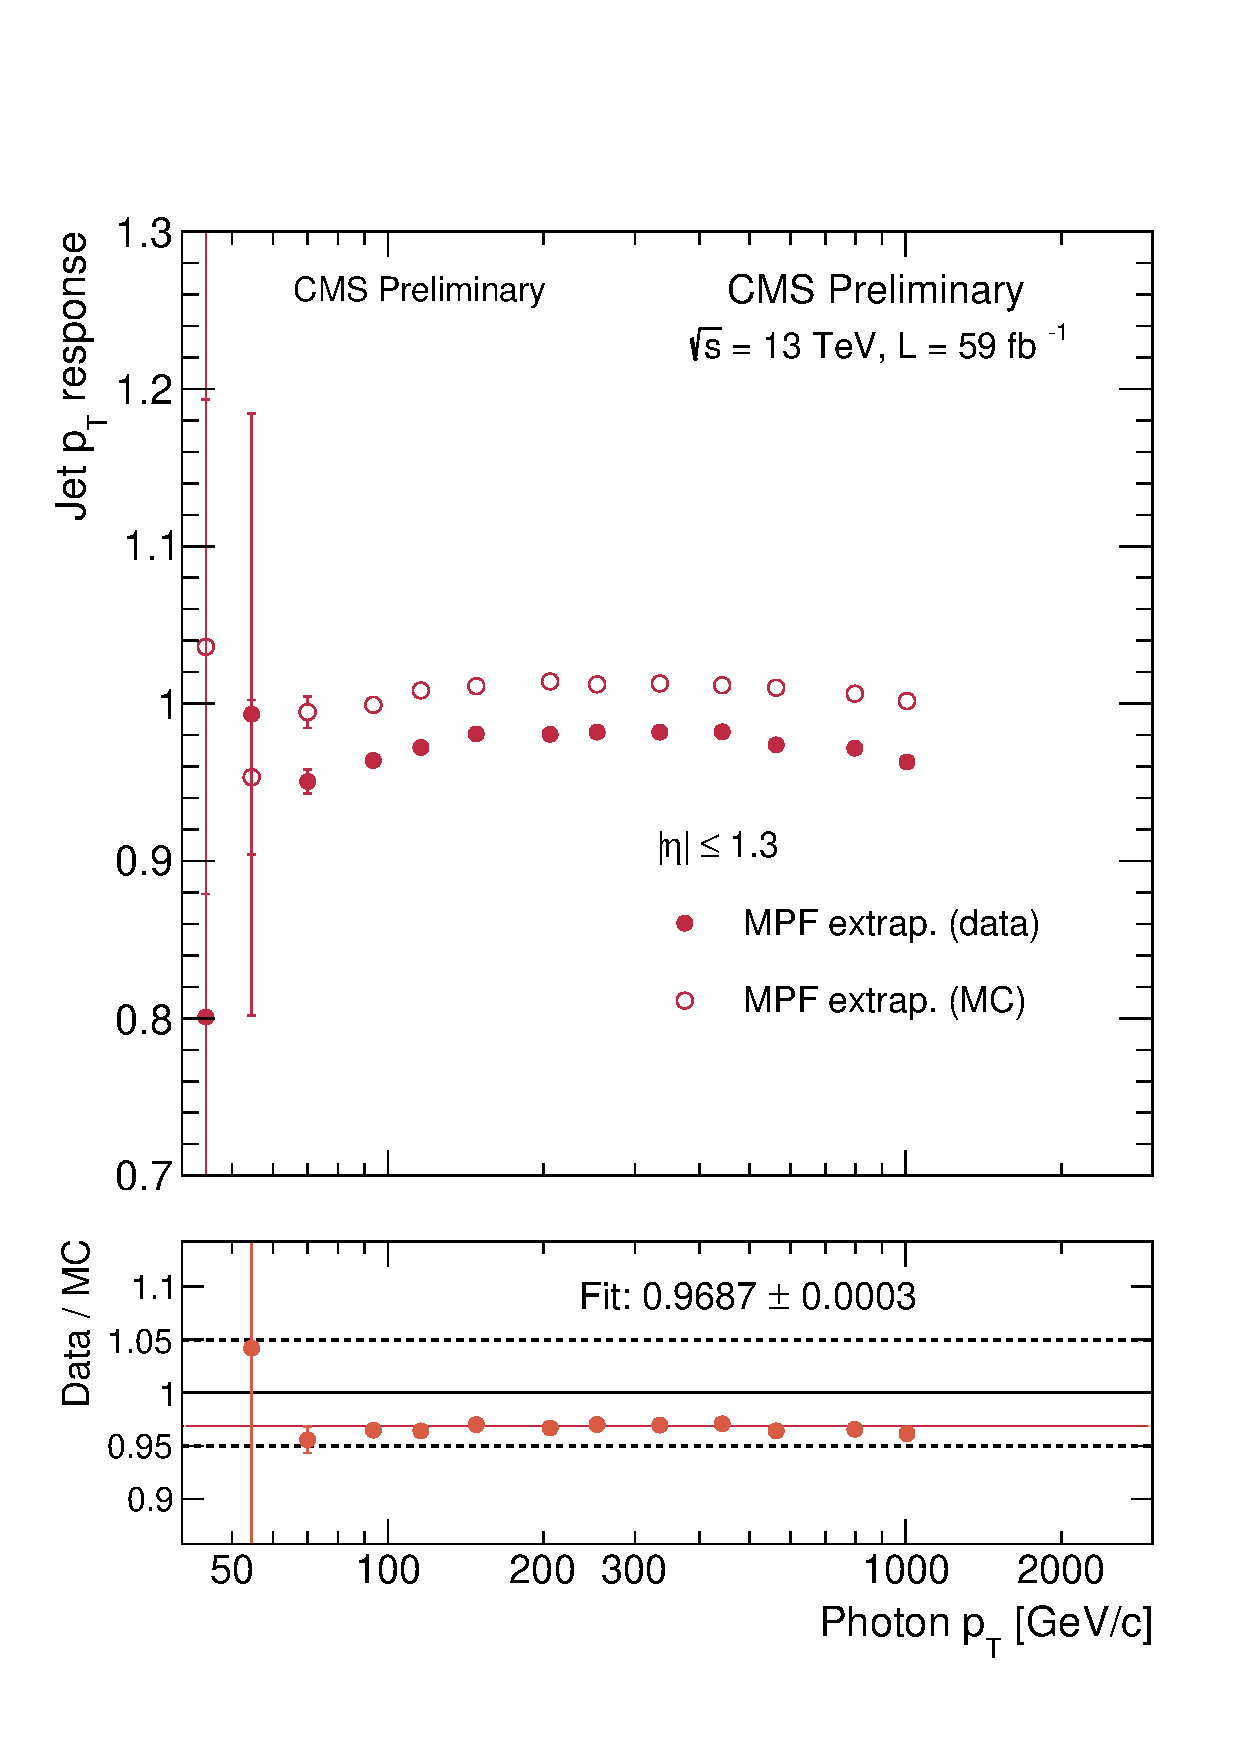
\includegraphics[width=.9\linewidth]{\PhDthesisdir/contents/chapter-JERC/plots/2019-07-25/only_L2Res/Run2018ABCD/extrapolated/response_eta0013_mpf_extrap.pdf}
\caption{MPF}
\end{figure}
\end{minipage}
\end{frame}

\subsection*{Correction de la résolution en énergie avec des événements \Gjets}
\begin{frame}
\frametitle{Jet Energy Resolution}
\manip Remember \Rbal\ definition,
\begin{equation*}
\Rbal = \frac{{\pT}^\text{1\up{st}jet}_\text{reco}}{\pT^\photon_\text{reco}}
\end{equation*}

\pause

Then
\begin{equation*}
\Rbal
=
\underbrace{\frac{{\pT}^\text{1\up{st}jet}_\text{reco}}{{\pT}^\text{1\up{st}jet}_\text{ptcl}}}_{\sigma_\text{jet}=\text{JER}}
\times
\underbrace{\frac{{\pT}^\text{1\up{st}jet}_\text{ptcl}}{\pT^\photon_\text{ptcl}}
\vphantom{\frac{{\pT}^\text{1\up{st}jet}_\text{reco}}{{\pT}^\text{1\up{st}jet}_\text{ptcl}}}}_{\text{PLI}}
\times
\underbrace{\frac{\pT^\photon_\text{ptcl}}{\pT^\photon_\text{reco}}
\vphantom{\frac{{\pT}^\text{1\up{st}jet}_\text{reco}}{{\pT}^\text{1\up{st}jet}_\text{ptcl}}}}_{\sigma_\photon\equiv1}
\end{equation*}
\manip PLI: Particle Level Imbalance (pile-up, radiations, neutrinos...), $\to0$ when $\alpha\to0$.

\pause
\begin{equation*}
\boxed{\text{JER} = \sigma_\text{jet} =  \sqrt{\sigma_\Rbal^2 - \sigma_\text{PLI}^2}}
\end{equation*}
\end{frame}


\begin{frame}
\frametitle{Run 2018 ABCD jet resolution}
\begin{minipage}{.45\textwidth}
\begin{figure}
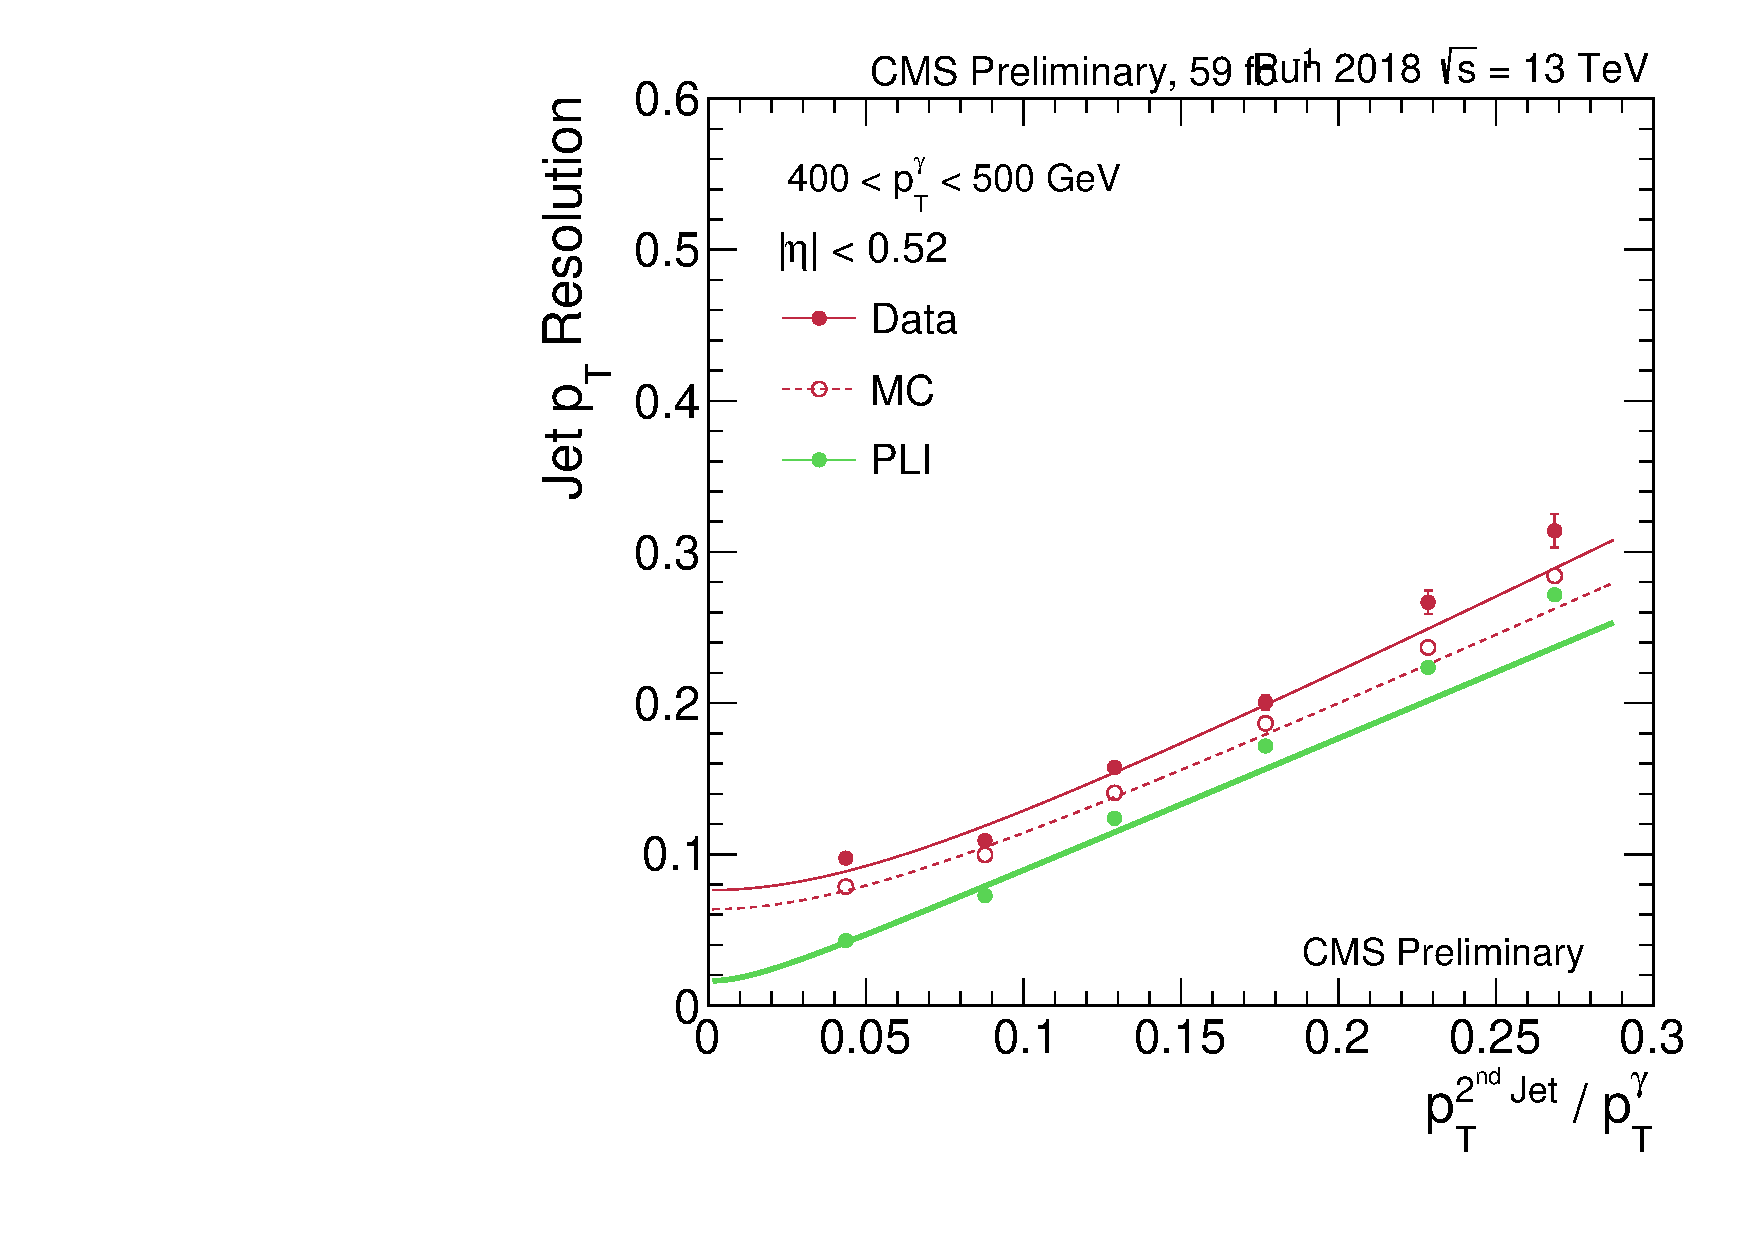
\includegraphics[width=\linewidth]{\PhDthesisdir/plots_and_images/my_plots/JERC/JER/Run2018ABCD/extrapolation/resolution_eta0005_ptPhot_400_500.pdf}
\caption{Extrapolation}
\end{figure}
\end{minipage}
\hfill
\begin{minipage}{.45\textwidth}
\begin{figure}
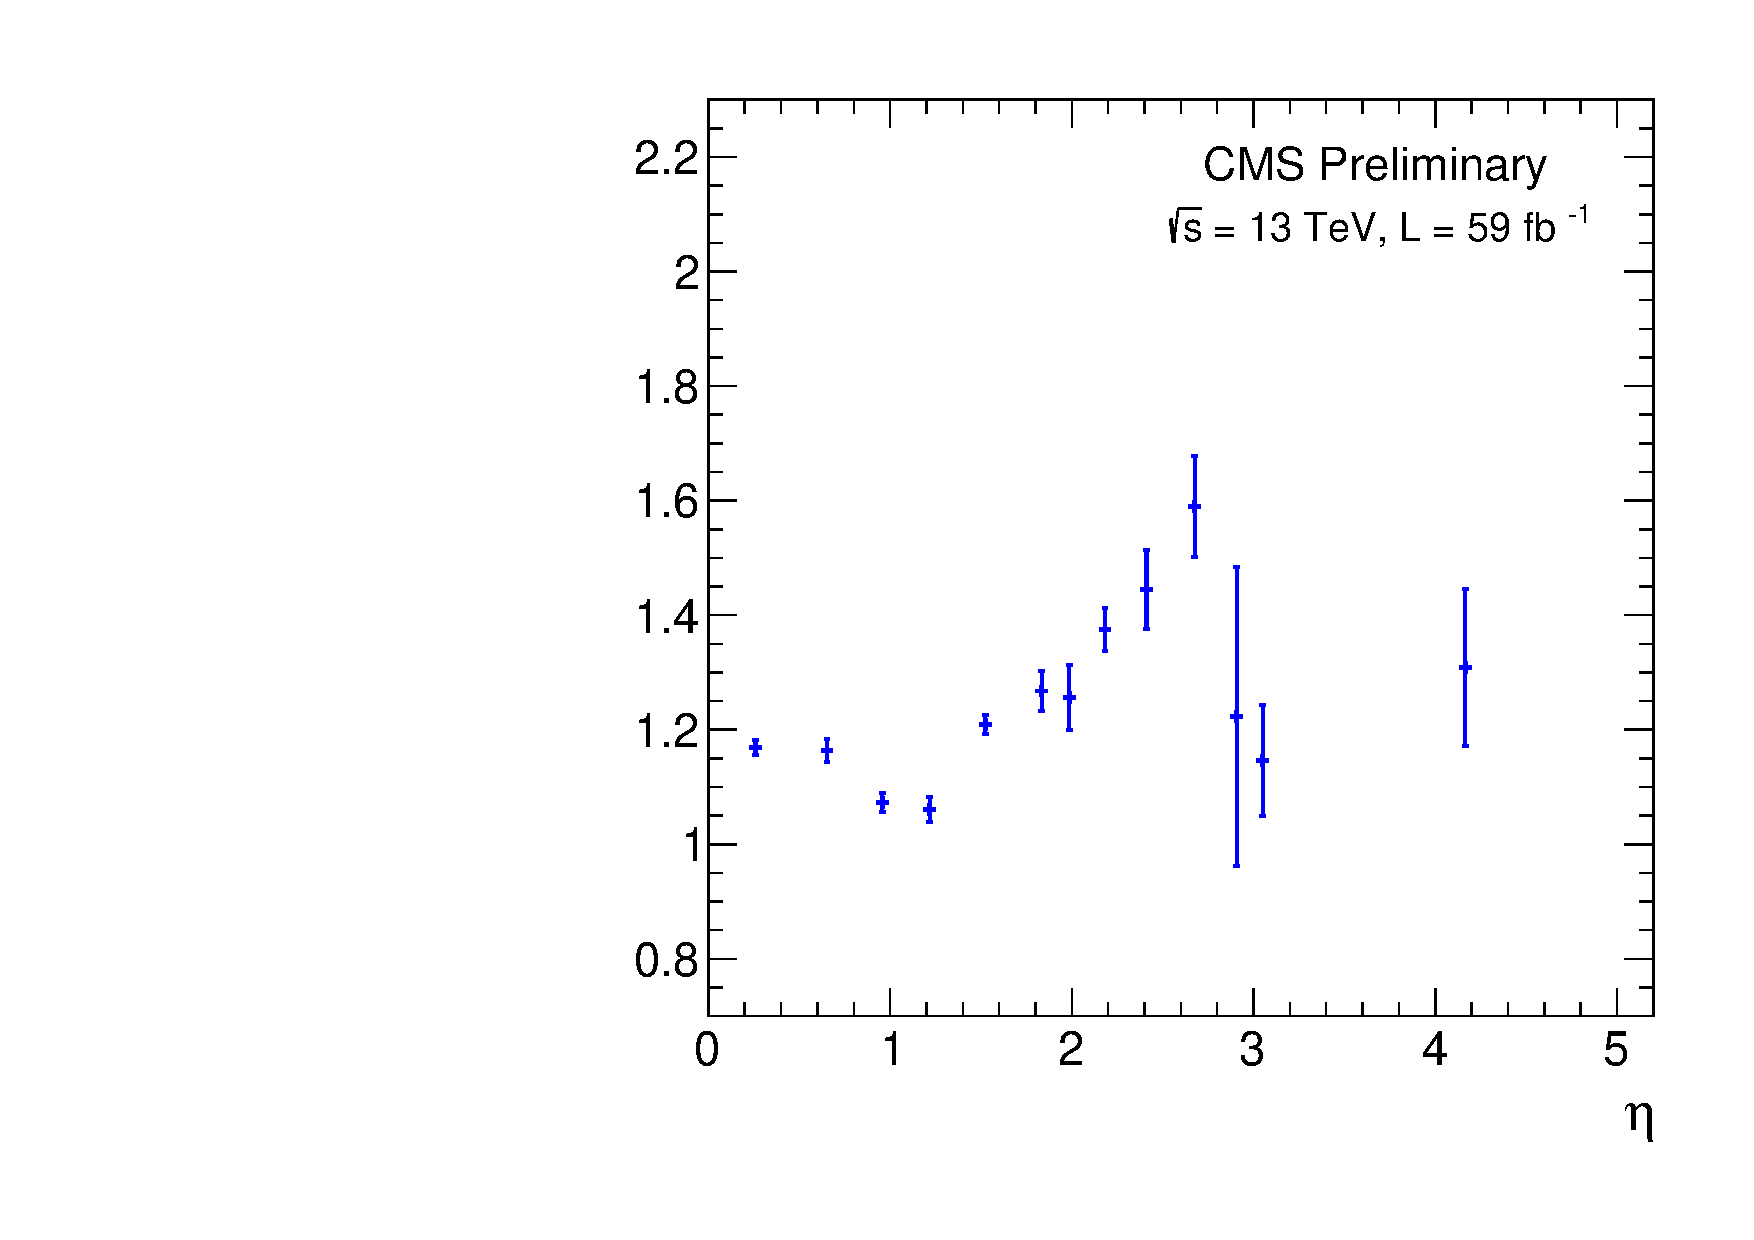
\includegraphics[width=\linewidth]{\PhDthesisdir/plots_and_images/my_plots/JERC/JER/Run2018ABCD/alpha_0_3/fine_eta_binning_Scale_factor_res_vs_ETA.pdf}
\caption{Scale factor}
\end{figure}
\end{minipage}
\end{frame}

\begin{frame}\addtocounter{framenumber}{-1}
\frametitle{Run 2018 ABCD jet resolution}
\begin{minipage}{.45\textwidth}
\begin{figure}
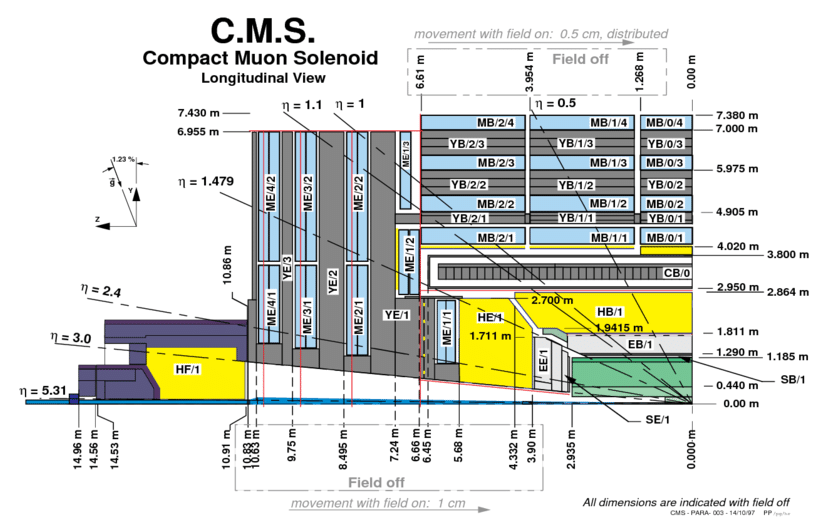
\includegraphics[width=\linewidth, trim=0cm 0cm 3cm 0cm]{\PhDthesisdir/plots_and_images/from_CMS_alignment_photodetectors/CMS-eta-ranges.png}
\caption{CMS and $\eta$ values}
\end{figure}
\end{minipage}
\hfill
\begin{minipage}{.45\textwidth}
\begin{figure}
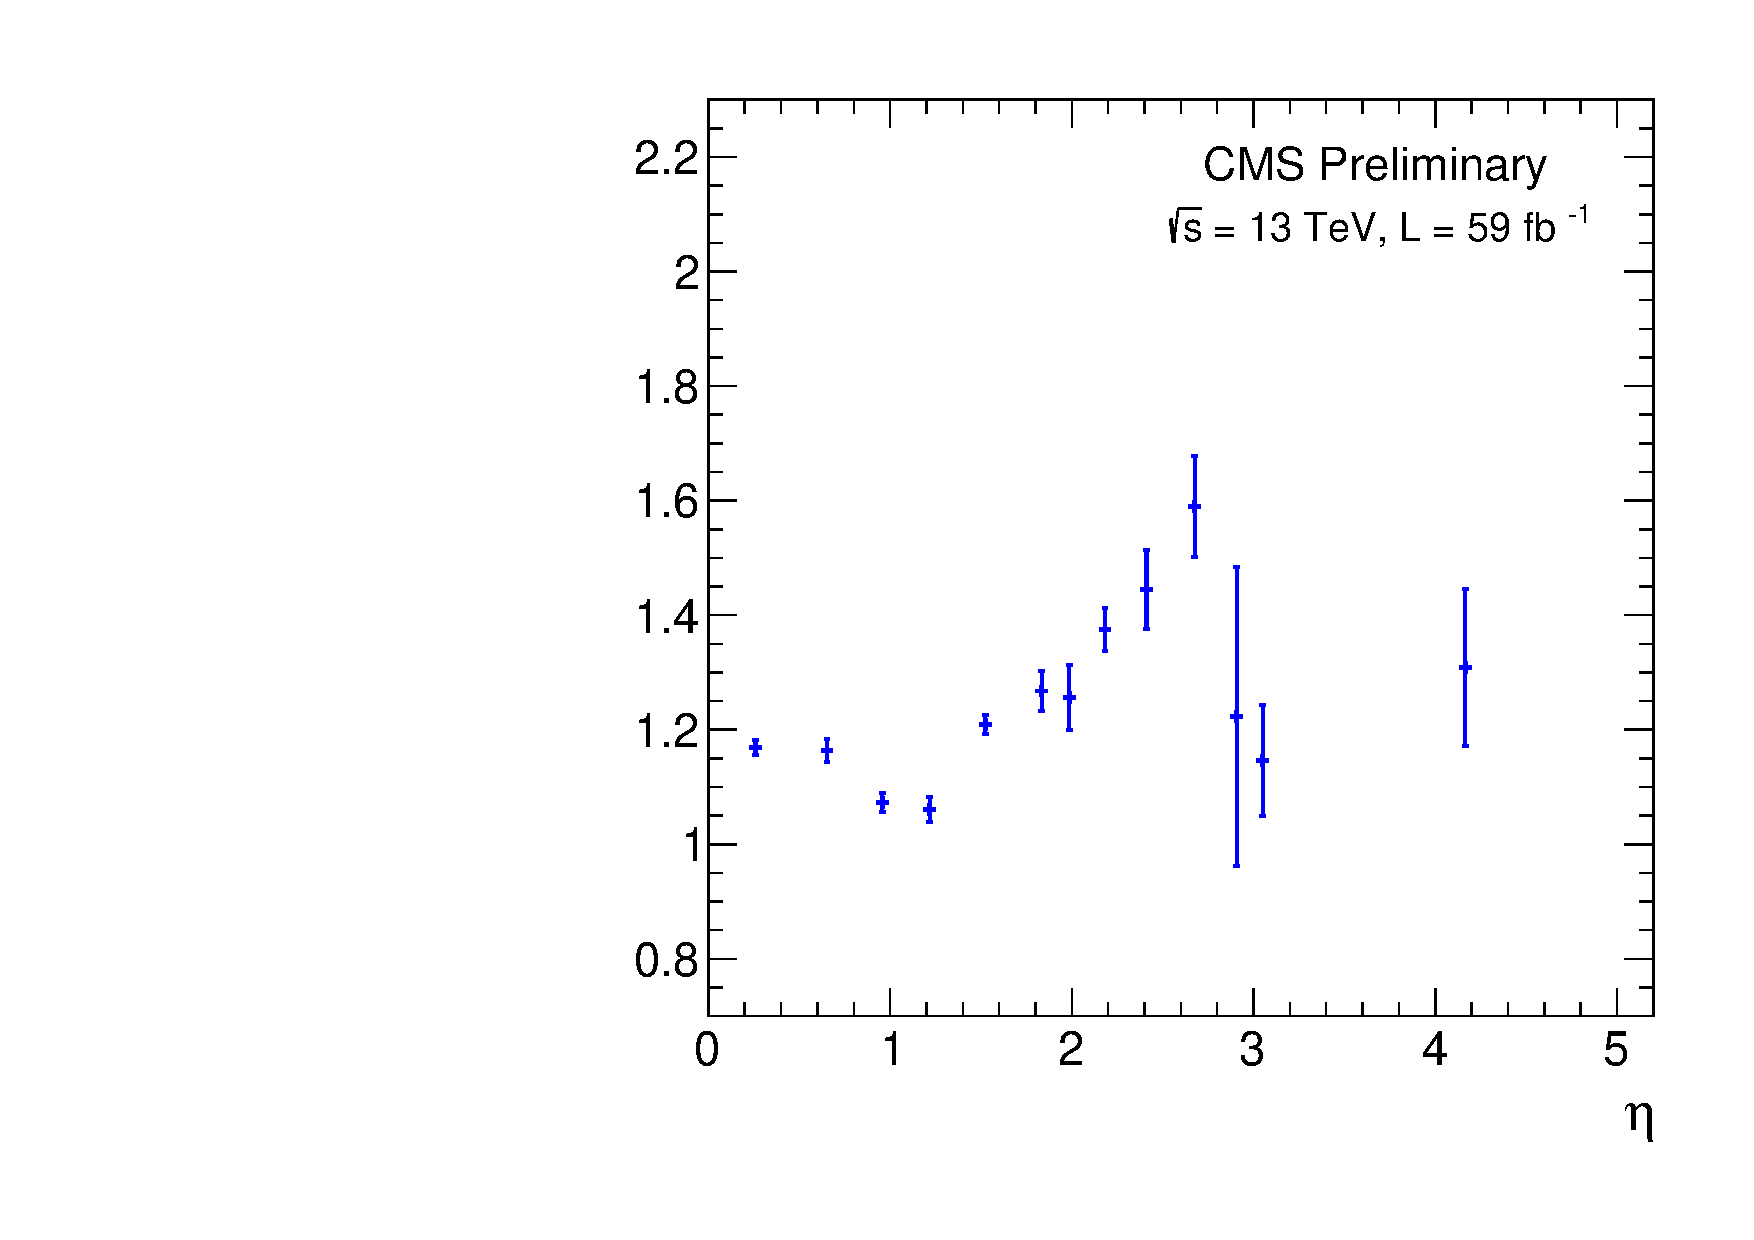
\includegraphics[width=\linewidth]{\PhDthesisdir/plots_and_images/my_plots/JERC/JER/Run2018ABCD/alpha_0_3/fine_eta_binning_Scale_factor_res_vs_ETA.pdf}
\caption{Scale factor}
\end{figure}
\end{minipage}
\end{frame}

